\documentclass[runningheads]{llncs}
%
\usepackage[T1]{fontenc}
% T1 fonts will be used to generate the final print and online PDFs,
% so please use T1 fonts in your manuscript whenever possible.
% Other font encondings may result in incorrect characters.
%
\usepackage{graphicx}
\usepackage{tikz}
\usepackage[inline]{enumitem}
\usepackage{pgf}
\usepackage{pgfplots}
\usepackage[hidelinks]{hyperref}
\usepackage{tcolorbox}
\usepackage{subcaption}
\usepackage{multirow}
\usepackage{amsfonts}
\usepackage{amsmath}
\usepackage{xspace}
\usepackage[ruled,vlined,linesnumbered]{algorithm2e}

\usepackage{booktabs}   % \toprule, \midrule, \bottomrule
\usepackage{multirow}   % \multirow
\usepackage{longtable}


\usetikzlibrary{positioning}

\usetikzlibrary{positioning}
\usetikzlibrary{ arrows.meta}
\usetikzlibrary{shapes.geometric}
\usetikzlibrary{calc}
\usetikzlibrary{arrows}
\usetikzlibrary{shapes, arrows, positioning, fit, calc, backgrounds, chains,decorations.pathreplacing,hobby}
\usetikzlibrary{mindmap,trees}
\usetikzlibrary{automata,positioning}
\usetikzlibrary{decorations.markings}


\usepackage{color}
\renewcommand\UrlFont{\color{blue}\rmfamily}


% Core mathematical notation.
\def\Gam{\ensuremath{\Gamma}\xspace}
\def\clockSet{\ensuremath{\mathcal{C}}\xspace}
\def\clockValuations#1{\ensuremath{\mathbb{R}_{\ge 0}^{#1}}\xspace}
\def\Nat{\ensuremath{\mathbb{N}}\xspace}
\def\Int{\ensuremath{\mathbb{Z}}\xspace}
\def\Reals{\ensuremath{\mathbb{R}}\xspace}
\def\kI{\ensuremath{I}\xspace}
\def\ck{\ensuremath{c}\xspace}
\def\DBM#1{\ensuremath{\mathbf{D}_{#1}}\xspace}
\def\UP{\ensuremath{\uparrow}\xspace}
\def\RESET#1{\ensuremath{[#1 \mathrel{:=} 0]}\xspace}
\def\tEU#1#2#3{\ensuremath{\mathrm{E}(#1\mathbf{U}_{#3}#2)}\xspace}
\def\tAU#1#2#3{\ensuremath{\mathrm{A}(#1\mathbf{U}_{#3}#2)}\xspace}
\def\EU#1#2{\ensuremath{\mathrm{E}(#1\mathbf{U}#2)}\xspace}
\def\AU#1#2{\ensuremath{\mathrm{A}(#1\mathbf{U}#2)}\xspace}
\def\EX#1{\ensuremath{\mathit{EX}#1}\xspace}
\def\AX#1{\ensuremath{\mathit{AX}#1}\xspace}
\def\tAR#1#2#3{\ensuremath{\mathrm{A}(#1\mathbf{R}_{#3}#2)}\xspace}
\def\tER#1#2#3{\ensuremath{\mathrm{E}(#1\mathbf{R}_{#3}#2)}\xspace}
\def\ER#1#2{\ensuremath{\mathrm{E}(#1\mathbf{R}#2)}\xspace}
\def\AR#1#2{\ensuremath{\mathrm{A}(#1\mathbf{R}#2)}\xspace}
\def\Z{\ensuremath{Z}\xspace}
\def\Deadline{\ensuremath{\mathcal{D}}\xspace}

% Rule-name helpers and clickable cross-references.
\makeatletter
\newcommand{\DeclareRule}[2]{\expandafter\def\csname rule@#1\endcsname{#2}}
\newcommand{\RuleLabel}[1]{{\ensuremath{#1}}}
\newcommand{\UunfRuleName}{\RuleLabel{\mathbf{U}^\bullet}}
\newcommand{\UstopRuleName}{\RuleLabel{\mathbf{U}\text{-stop}}}
\newcommand{\UgoRuleName}{\RuleLabel{\mathbf{U}\text{-go}}}
\newcommand{\UgoCarryRuleName}{\RuleLabel{\mathbf{U}^\ast\text{-go}}}
\newcommand{\RsplitRuleName}{\RuleLabel{\mathbf{R}^{\mathsf{split}}}}
\newcommand{\RbranchName}[1]{\RuleLabel{\mathbf{R}^\bullet_{#1}}}
\newcommand{\RbranchStopName}[1]{\RuleLabel{\mathbf{R}^\bullet_{#1}\text{-stop}}}
\newcommand{\RbranchGoName}[1]{\RuleLabel{\mathbf{R}^\bullet_{#1}\text{-go}}}
\newcommand{\rulename}[1]{\ensuremath{(\csname rule@#1\endcsname)}}
\newcommand{\ruleanchor}[1]{\hypertarget{rule:#1}{\rulename{#1}}}
\newcommand{\ruleref}[1]{\ifcsname r@tag:#1\endcsname\hyperref[tag:#1]{\rulename{#1}}\else\hyperlink{rule:#1}{\rulename{#1}}\fi}
\newcommand{\rname}[1]{\csname rule@#1\endcsname}
\newcommand{\rlink}[1]{\ifcsname r@tag:#1\endcsname\hyperref[tag:#1]{\rulename{#1}}\else\hyperlink{rule:#1}{\rulename{#1}}\fi}
\makeatother
\DeclareRule{AND}{\land}
\DeclareRule{OR}{\lor}
\DeclareRule{AX}{\mathrm{AX}}
\DeclareRule{EX}{\mathrm{EX}}
\DeclareRule{Delay}{\mathrm{Delay}}
\DeclareRule{Conj}{\land}
\DeclareRule{Disj}{\lor}
\DeclareRule{Cov}{\mathrm{Cov}}
\DeclareRule{Covstar}{\mathrm{Cov}^{*}}
\DeclareRule{Uunf}{\UunfRuleName}
\DeclareRule{Runf}{\mathbf{R}^\bullet}
\DeclareRule{Rsplit}{\RsplitRuleName}
\DeclareRule{Runf_before}{\RbranchName{\prec\kI}}
\DeclareRule{Runf_in}{\RbranchName{\in\kI}}
\DeclareRule{Runf_after}{\RbranchName{\succ\kI}}
\DeclareRule{Runf_lapse}{\RuleLabel{\mathbf{R}^\bullet_{\succ\kI}^{\mathsf{lapse}}}}
\DeclareRule{Ustop}{\UstopRuleName}
\DeclareRule{Ugo}{\UgoRuleName}
\DeclareRule{Ugocarry}{\UgoCarryRuleName}
\DeclareRule{Rbeforestop}{\RbranchStopName{\prec\kI}}
\DeclareRule{Rbeforego}{\RbranchGoName{\prec\kI}}
\DeclareRule{Rinstop}{\RbranchStopName{\in\kI}}
\DeclareRule{Ringo}{\RbranchGoName{\in\kI}}
\DeclareRule{Rstop}{\RuleLabel{\mathbf{R}^\bullet\text{-stop}}}
\DeclareRule{Rgo}{\RuleLabel{\mathbf{R}^\bullet\text{-go}}}
\DeclareRule{discharge}{\mathsf{discharge}}
\DeclareRule{launch}{\mathsf{launch}}
\DeclareRule{Rsplitbefore}{\RbranchName{\prec\kI}}
\DeclareRule{Rsplitin}{\RbranchName{\in\kI}}
\DeclareRule{Rsplitafter}{\RbranchName{\succ\kI}}
\DeclareRule{openseg}{\mathsf{open seg.}}
\DeclareRule{boundary}{\mathsf{boundary}}




% Figure helpers.
\newcommand{\myvdots}[4]{%
  % #1 = x-coordinate
  % #2 = y-coordinate of top dot
  % #3 = vertical spacing
  % #4 = dot radius
  \foreach \i [evaluate=\i as \yy using #2-\i*#3] in {0,1,2}
    \fill (#1,\yy) circle[radius=#4];
}

\newcommand{\lemitem}[2]{\hyperref[#1]{\ref*{#1}(\textup{#2})}}

% Shared shorthand commands live in acronyms.tex.
% Acronyms and shorthand commands used across the manuscript.
% Keeping these separate makes the main preamble easier to scan and maintain.

% Semantic shorthands used in the prose.
\providecommand{\eventualities}{\ensuremath{\mathcal{E}}\xspace}
\providecommand{\obligations}{\ensuremath{\mathcal{O}}\xspace}
\providecommand{\ctx}{\ensuremath{\mathit{ctx}}\xspace}
\providecommand{\INF}{\ensuremath{\infty}\xspace}
\providecommand{\SAT}{\ensuremath{\mathrm{SAT}}\xspace}
\providecommand{\UNSAT}{\ensuremath{\mathrm{UNSAT}}\xspace}
\providecommand{\EF}{\ensuremath{\mathrm{EF}}\xspace}
\providecommand{\AF}{\ensuremath{\mathrm{AF}}\xspace}
\providecommand{\EG}{\ensuremath{\mathrm{EG}}\xspace}
\providecommand{\AG}{\ensuremath{\mathrm{AG}}\xspace}
\providecommand{\OPEN}{\ensuremath{\checkmark}\xspace}
\providecommand{\CLOSED}{\ensuremath{\times}\xspace}
\providecommand{\UNKNOWN}{\ensuremath{\mathsf{Unknown}}\xspace}
\providecommand{\file}[1]{\ensuremath{\texttt{#1}}\xspace}
\providecommand{\func}[1]{\ensuremath{\texttt{#1()}}\xspace}
\providecommand{\Zuniv}{\ensuremath{\top}\xspace}
\providecommand{\Sub}[1]{\ensuremath{\mathit{Sub}(#1)}\xspace}
\providecommand{\Zone}{\ensuremath{\mathcal{Z}}\xspace}
\providecommand{\Ctx}{\ensuremath{\mathcal{X}}\xspace}
\providecommand{\TabGraph}{\ensuremath{\mathcal{G}_{\varphi}}\xspace}
\providecommand{\TabNode}{\ensuremath{\mathcal{N}_{\varphi}}\xspace}
\providecommand{\TabEdge}{\ensuremath{\mathcal{E}_{\varphi}}\xspace}
\providecommand{\nxQ}{\ensuremath{\mathsf{X}_{\mathrm{Q}}}\xspace}
\providecommand{\Sat}{\ensuremath{\mathcal{S}}\xspace}
\providecommand{\FormalSmaller}{\ensuremath{\prec}\xspace}
\providecommand{\tup}[5]{\ensuremath{\langle #1, #2, #3, #4, #5\rangle}\xspace}
\providecommand{\psiU}{\ensuremath{\tEU{p}{q}{[1,2]}}\xspace}
\providecommand{\psiR}{\ensuremath{\tAR{\bot}{p}{[0,1]}}\xspace}
\providecommand{\psiG}{\ensuremath{\AR{\bot}{p}}\xspace}

% Tableau markers and recurring derived notation.
\providecommand{\ANDn}{\ensuremath{\otimes}}
\providecommand{\ORn}{\ensuremath{\oplus}}
\providecommand{\DETn}{\ensuremath{\odot}}
\providecommand{\rst}[2]{#1[#2\,{:=}\,0]}
\providecommand{\kJ}{\ensuremath{J}\xspace}
% Recurrence window of a persistent pursuit: I at the first witness, [0,b-a] after.
\providecommand{\kIrec}{\ensuremath{I^{\ast}}\xspace}
\providecommand{\Inv}{\mathsf{Inv}}
\providecommand{\cvx}{\mathsf{cvx}}
\providecommand{\ZltI}{Z^{\prec\kI}}
\providecommand{\ZinI}{Z^{\in\kI}}
\providecommand{\ZgtI}{Z^{\succ\kI}}
\providecommand{\Dopen}{\Delta^{\circ}}
\providecommand{\Dbd}{\Delta^{\partial}}
\providecommand{\dom}{\operatorname{dom}}
\providecommand{\kind}{\mathit{kind}}
\providecommand{\Acc}{\mathit{Acc}}
\providecommand{\Rej}{\mathit{Rej}}
\providecommand{\FL}{\mathsf{FL}}
\providecommand{\Subt}{\mathsf{T}}

% Algorithm-state shorthands.
\providecommand{\val}{\mathit{val}}
\providecommand{\idx}{\mathit{idx}}
\providecommand{\low}{\mathit{low}}
\providecommand{\onstk}{\mathit{on}}
\providecommand{\ch}{\mathit{ch}}
\providecommand{\Stack}{\mathcal{S}}
\providecommand{\cnt}{\mathit{c}}
\providecommand{\Out}{\mathit{Out}}


%%%%%%%%%%%%%%%%%%%%%%%%%%%%%%%%%%%%%%%%%%%%%%%%%%%%%%%%%%%%%%%%%%%%%%%%%%%%%%
%% Algorithm procedure names.
%% Declared after algorithm2e is loaded so the names type consistently in
%% both the algorithm listings and the prose that refers to them.
%%%%%%%%%%%%%%%%%%%%%%%%%%%%%%%%%%%%%%%%%%%%%%%%%%%%%%%%%%%%%%%%%%%%%%%%%%%%%%
\SetKwFunction{Decide}{Decide}
\SetKwFunction{Explore}{Explore}
\SetKwFunction{Eliminate}{Eliminate}
\SetKwFunction{Expand}{Expand}
\SetKwFunction{Settles}{Settles}
\SetKwFunction{Retire}{Retire}

% Rule keys this presentation adds; the rest are declared in preamble.tex.
\DeclareRule{Carry}{\mathrm{Carry}}
\DeclareRule{Absorb}{\mathrm{Abs}}
\DeclareRule{Umiss}{\mathbf{U}\text{-miss}}
\newcommand{\UstopCarryRuleName}{\mathbf{U}^{\ast}\text{-stop}}
\newcommand{\UunfCarryRuleName}{\mathbf{U}^{\ast}}
\DeclareRule{Ustopcarry}{\UstopCarryRuleName}
\DeclareRule{Uunfcarry}{\UunfCarryRuleName}


%% Algorithms 1 and 2 are tall floats; the LaTeX defaults defer anything over
%% 70% of the text height to a float page at the end of the document, which put
%% them eleven pages after the text that refers to them.
%\renewcommand{\topfraction}{0.92}
%\renewcommand{\bottomfraction}{0.85}
%\renewcommand{\textfraction}{0.06}
%\renewcommand{\floatpagefraction}{0.7}
%\setcounter{topnumber}{3}
%\setcounter{totalnumber}{5}


\urlstyle{rm}
%
\begin{document}

\title{A Tableau for TCTL}

\titlerunning{A Tableau for TCTL}

\author{Luca Brodo\orcidID{0009-0005-1437-9861} \and
Giuseppe Scalora\orcidID{0009-0005-3163-82634} \and
Stefan Henkler\orcidID{0009-0000-4979-9456}}
%
\authorrunning{L. Brodo et al.}
% First names are abbreviated in the running head.
% If there are more than two authors, 'et al.' is used.
%
\institute{Hochschule Hamm-Lippstadt, Germany \\
\email{\{name.last\_name\}@hshl.de}\\
}
%
\maketitle              % typeset the header of the contribution
%
\begin{abstract}

We present the first tableau-based decision procedure for the satisfiability problem of Timed
Computation Tree Logic (TCTL). Our approach is an on-the-fly, symbolic proof search that explores only the relevant part of the state space and excludes spurious Zeno witnesses, so that for every satisfiable formula it yields a realisable timed automaton as a certificate of satisfiability. Our procedure is sound and terminating for the general TCTL, and complete for its non-punctual fragment, where it matches the optimal \textsc{ExpTime} bound. Our evaluation shows that it remains feasible in practice, even for formulas with a large number of nested temporal operators, with a consistently low, almost-flat cost for the kind of TCTL properties engineers write in practice.

\keywords{TCTL  \and Satisfiability \and Real-Time Systems }
\end{abstract}
\section{Introduction}\label{sec:intro}

%The severe consequences of software failures in safety-critical domains necessitate rigorous verification workflows to establish system correctness. Model-checking is the established approach for this purpose~\cite{Baier08,Clarke99}. 


%The model-checking workflow typically involves formalizing system requirements in a temporal logic and automatically verifying a formal model of the system against these specifications. In the context of real-time systems, where correctness depends not only on functional behaviour but also on timing, this workflow is commonly instantiated using timed automata~\cite{AlurDill1994} as the modelling formalism, Timed Computation Tree Logic (TCTL)~\cite{AlurCourcoubetisDill1990} as the specification language, and \textsc{Uppaal}~\cite{BehrmannLarsenYi2004Uppaal} as the verification tool, as demonstrated in various applications~\cite{Guo2014UPPAAL,Laursen2020Railway,Mikucionis2010Herschel}.



Establishing the correctness of safety-critical software is a central concern of formal verification, for which model checking is the established approach~\cite{Baier08,Clarke99}. For real-time systems, where correctness depends not only on functional behaviour but also on timing, software is typically modelled as a timed automaton (TA)~\cite{AlurDill1994} and verified against requirements expressed in Timed Computation Tree Logic (TCTL)~\cite{AlurCourcoubetisDill1990} using efficient tools such as \textsc{Uppaal}~\cite{BehrmannLarsenYi2004Uppaal}, as exemplified by~\cite{Guo2014UPPAAL,Laursen2020Railway,Mikucionis2010Herschel}. 


In this workflow, however, the verification step only establishes conformance between a system and a specification; it says nothing about the quality of the specification itself. A TCTL property may be unsatisfiable, valid or refined by another property in the sense of~\cite{10.1145/3808127,BrodoScaloraHenkler2026MinimalTemporalProperties}. Each of these defects is ultimately a question of satisfiability, and detecting them therefore requires a satisfiability procedure for TCTL. 


The satisfiability problem for TCTL is known to be undecidable in
general~\cite{AlurCourcoubetisDill1990,AlurHenzinger1994ReallyTemporal}. Finite
satisfiability is nonetheless recursively
enumerable, so enumerating candidate automata and model checking each is sound
and eventually finds a model for every satisfiable formula; it simply never
terminates on an unsatisfiable one. La~Torre and
Napoli~\cite{fsttcs2000-LN,LaTorreNapoli2001TimedTreeAutomata} traced the source
of undecidability to punctuality, showing that once singular intervals are
forbidden, i.e., in the \emph{non-punctual} fragment, finite satisfiability
becomes decidable in \textsc{ExpTime} by reduction to emptiness of timed tree
automata, at the cost of a global construction, exponential in the formula. Subsequent work traded completeness
for implementability: Penczek et al.~\cite{boundedTCTL} reduce satisfiability to
the existence of a \emph{bounded} parametric TA, instantiated with
\textsc{Imitator}~\cite{imitator3}; their method is sound but incomplete, does not
handle nested modalities, and terminates by virtue of the imposed bound.

To this day, no search-based, goal-directed procedure for TCTL satisfiability has been proposed, and the only practical approach is bounded and partial. 

%To fill this gap, we present the first on-the-fly, symbolic and tableau-based decision procedure for satisfiability of TCTL. Contrary to previous work, not only is our procedure sound and complete for the non-punctual fragment, but it is also sound and terminating for the general TCTL as well as complete for TCTL formulae of temporal nesting equal to 1, thus deciding the typical properties engineers write in practice. Moreover, our procedure is directly implementable, matches the optimal \textsc{ExpTime} bound~\cite{LaTorreNapoli2001TimedTreeAutomata}, and returns a witnessing TA whenever the input formula is satisfiable.
%
%

To fill this gap, we present the first on-the-fly, symbolic and tableau-based
decision procedure for satisfiability of TCTL. Unlike previous work, not only is our procedure sound, but also terminating for the general TCTL. On the non-punctual fragment the procedure is in
addition complete, matching the optimal \textsc{ExpTime}
bound~\cite{Clarke99,fsttcs2000-LN}. Completeness moreover extends
beyond that fragment, to every formula of temporal nesting depth~1, punctuality
included, thus deciding most of the typical properties engineers write in practice. Finally, our procedure is directly implementable, matches the optimal \textsc{ExpTime} bound~\cite{LaTorreNapoli2001TimedTreeAutomata}, and returns a witnessing TA whenever the input formula is satisfiable.

Unlike the classical tableau constructions for logics such as CTL or
\emph{discrete}-time quantitative CTL~\cite{tableau_ctl,Clarke99,EmersonEtAl1992QuantitativeTemporalReasoning},
our calculus must contend with two phenomena of the {dense-time} semantics.
First, \emph{zenoness}: a cycle may be traversed infinitely often within a bounded
total delay, so a branch defers a deadline for ever without ever reaching it, along a
run no system exhibits. Second, an eventuality under a $\mathrm{AG}$ is demanded
at a continuum of instants, each carrying its own deadline. We settle the first with an
acceptance condition on the tableau graph itself, and the second by covering the continuum symbolically.

We structure the paper as follows.  Section~\ref{sec:back} presents the background; Section~\ref{sec:tableau} presents our procedure; Section~\ref{sec:correct} establishes
termination, soundness, completeness, and complexity; Section~\ref{sec:eval} evaluates a prototype.




%
%\section{Related Work}\label{sec:related_work}
%
%
%Tableau methods are classical for untimed branching-time logics~\cite{Clarke99,tableau_ctl}, but handle neither dense clocks nor Zeno behaviour. The closest tableau in spirit targets a \emph{discrete}-time quantitative CTL~\cite{EmersonEtAl1992QuantitativeTemporalReasoning}, which, however, does not hanlde dense-time phenomena. 
%
%The only other decision procedure for non-punctual TCTL is the one proposed in~\cite{fsttcs2000-LN,LaTorreNapoli2001TimedTreeAutomata}, who settle its decidability with the same \textsc{ExpTime} bound. Their route is automata-theoretic and global: the formula is translated as a whole into a timed tree automaton and satisfiability is reduced to emptiness. This monolithic construction affords no goal-directed exploration and does not directly yield the TA \emph{system} model that verification tools consume. We instead obtain such a model directly: our tableau stays at the logical level throughout, building only the demanded fragment of the state space, maintaining clock valuations symbolically as zones, excluding Zeno witnesses explicitly, and extracting a concrete TA from a successful derivation.
%
%A synthesis-oriented alternative is the bounded method of Penczek et al.~\cite{boundedTCTL}, which reduces TCTL satisfiability to the existence of a bounded parametric TA, instantiated through the \textsc{Imitator}~\cite{imitator3} model checker. There, termination stems from an imposed structural bound rather than from the logic of the
%procedure, so the method is inherently incomplete; and the fragment it addresses is incomparable
%to ours, forbidding nesting yet admitting punctual constraints, for which satisfiability is
%undecidable. Ours is the maximal \emph{decidable} fragment, which we decide completely, and our
%calculus runs soundly on punctual input as well, so the two fragments are covered by one
%procedure at differing guarantees.
%



\section{Background}\label{sec:back}

%We fix a finite set $\mathcal{P}$ of atomic propositions and a finite set $\clockSet$ of {clocks}, that is real-valued variables that increase uniformly with time. 
 
A {time bound} $\kI$ is a non-empty interval of $\mathbb{R}_{\ge 0}$ with integer endpoints of the form $[a,b],(a,b],[a,b),(a,b)$ with $a\le b$, $a\in\Int_{\ge0}$, $b\in\Int_{\ge0}\cup\{\infty\}$. Non-emptiness leaves $[a,a]$ as the only bound with $a=b$; we call it \emph{punctual}.

%We only consider non-punctual bounds, so $[a,a]$ is excluded.
Fix a finite set $\mathcal{P}$ of atomic propositions. We study TCTL in negation normal form over these time bounds, built according to the following grammar:
%We study TCTL in negation normal form over the non-punctual fragment, built from two timed path modalities, {until} and {release}:
\vspace{-0.1cm}
\[
\varphi ::= \top \mid \bot \mid p \mid \neg p \mid \varphi\land\varphi \mid \varphi\lor\varphi \mid
\mathrm{E}(\varphi\mathbf{U}_\kI\varphi) \mid \mathrm{E}(\varphi\mathbf{R}_\kI\varphi) \mid \mathrm{A}(\varphi\mathbf{U}_\kI\varphi) \mid \mathrm{A}(\varphi\mathbf{R}_\kI\varphi).
\]

Other operators are expressible by the grammar: $\mathrm{EF}_\kI \varphi \equiv \mathrm{E}(\top\mathbf{U}_\kI\varphi)$, $\mathrm{AF}_\kI \varphi \equiv \mathrm{A}(\top\mathbf{U}_\kI\varphi)$, $\mathrm{EG}_\kI \varphi \equiv \mathrm{E}(\bot\mathbf{R}_\kI\varphi)$, and $\mathrm{AG}_\kI \varphi \equiv \mathrm{A}(\bot\mathbf{R}_\kI\varphi)$. 
%Every other operator can be directly established through this grammar: $\mathrm{F}_\kI\varphi\equiv\top\mathbf{U}_\kI\varphi$ and $\mathrm{G}_\kI\varphi\equiv\bot\mathbf{R}_\kI\varphi$. Prefixed
%by a path quantifier these give the familiar $\mathrm{EF}_\kI,\mathrm{AF}_\kI$ -- shorthand for
%$\mathrm{E}(\top\mathbf{U}_\kI\cdot)$ and $\mathrm{A}(\top\mathbf{U}_\kI\cdot)$ -- and dually
%$\mathrm{EG}_\kI,\mathrm{AG}_\kI$ for $\mathrm{E}(\bot\mathbf{R}_\kI\cdot)$ and
%$\mathrm{A}(\bot\mathbf{R}_\kI\cdot)$; the {untimed} operators are the case $\kI=[0,\infty)$. 
Unlike CTL the logic has {no next operator}:
over dense time no configuration has an immediate successor~\cite{AlurCourcoubetisDill1990}. The symbols $\EX,\AX$ used by the tableau are proof-theoretic
markers internal to the construction, never object operators. 
Throughout, we consider a formula $\varphi$ of size $n=|\FL(\varphi)|$, where $\FL(\varphi)$ is its Fischer--Ladner closure.

TCTL is interpreted over the timed transition system (TTS) induced by a TA~\cite{AlurCourcoubetisDill1990,Baier08}. A TA~\cite{BehrmannLarsenYi2004Uppaal,Bouyer05TimedAutomata} over set of clocks $\clockSet$ is a tuple $\mathcal{A}=\langle S,s_0,\mathsf{Inv},E,\mathcal{P},L\rangle$:
locations $S$, initial $s_0$, a {location invariant} $\mathsf{Inv}(s)$ (that is, a downward-closed constraint on clock valuations), discrete edges
$E\subseteq S\times 2^{\clockSet}\times S$ (each carrying the clocks it resets), and a labelling
$L:S\to 2^{\mathcal{P}}$.  An
invariant bounds how long time may elapse in a location: without it a run could idle in a location forever. Invariant-free locations are allowed, so the model expresses idling as well. $\mathcal{A}$ is {non-blocking} (time can always
diverge, hence no timelock). 

Any $\mathcal{A}$ induces a TTS $\mathcal{T}=\langle C,c_0,\xrightarrow{\cdot},\to\rangle$, whose configurations $C=\{(s,\nu)\in S\times\clockValuations{\clockSet}\mid \nu\models\mathsf{Inv}(s)\}$ pair a location with an admissible clock valuation, and whose initial configuration is $c_0=(s_0,\mathbf{0})$. Two relations act on configurations: $\xrightarrow{\ \cdot\ } \subseteq C\times\mathbb{R}_{\ge0}\times C$, the delay relation, which we write $(s,\nu)\xrightarrow{t}(s,\nu+t)$ for $t\in\mathbb{R}_{\ge0}$ such that $\nu+t'\models\mathsf{Inv}(s)$ throughout $t'\in[0,t]$; and $\to\subseteq C\times C$, the discrete relation, which we write $(s,\nu)\to(s',\nu[R:=0])$ for each edge $(s,R,s')\in E$ with $\nu\models\mathsf{Inv}(s)$ and $\nu[R:=0]\models\mathsf{Inv}(s')$, where the \emph{reset} $\nu[R:=0]$ zeroes every clock in $R\subseteq \clockSet$ and leaves the others unchanged. 
%(i.e.\ $\nu[R:=0](x)=0$ if $x\in R$, and $\nu(x)$ otherwise).



A {run} $\rho$ from any $c\in C$ is a maximal alternation of delays $t_0,t_1,\dots$ and discrete steps; a
{position} $\pi=(i,\delta)$ with $0\le\delta\le t_i$ denotes the configuration $\rho(\pi)$ after the $i$-th
discrete step plus delay $\delta$, at elapsed time $\mathit{time}(\pi)=T_i+\delta$ (with
$T_i=\sum_{j<i}t_j$), positions ordered by the lexicographic $\preceq$. The run is {non-Zeno} when its delays sum to $\infty$; by non-blockingness the set
$\mathrm{Runs}^\infty(c)$ of non-Zeno runs is non-empty. The TCTL satisfaction relation is the standard
one~\cite{AlurCourcoubetisDill1990}, evaluated over $\mathrm{Runs}^\infty$; for a single run, timed until and release read:
\vspace{-0.2cm}
\begin{align}
\rho&\models\varphi\mathbf{U}_\kI\psi \iff
\exists\pi\big[\mathit{time}(\pi)\in\kI \wedge \rho(\pi)\models\psi \wedge
\forall\pi'\prec\pi(\rho(\pi')\models\varphi)\big]
\label{eq:sat_u}\\
\rho&\models\varphi\mathbf{R}_\kI\psi \iff
\forall\pi\big[\mathit{time}(\pi)\in\kI \Rightarrow
\big(\rho(\pi)\models\psi \vee \exists\pi'\prec\pi(\rho(\pi')\models\varphi)\big)\big]
\label{eq:sat_r}
    \end{align}

%at the level of a single run the
%timed until reads
%\begin{equation}
%\rho\models\varphi\mathbf{U}_\kI\psi \iff
%\exists\pi\big[\mathit{time}(\pi)\in\kI \wedge \rho(\pi)\models\psi \wedge
%\forall\pi'\prec\pi(\rho(\pi')\models\varphi)\big],
%\label{eq:sat_u}
%\end{equation}
%and release is its dual, $\varphi\mathbf{R}_\kI\psi\equiv\neg(\neg\varphi\mathbf{U}_\kI\neg\psi)$, or equivalently
%\begin{equation}
%\rho\models\varphi\mathbf{R}_\kI\psi \iff
%\forall\pi\big[\mathit{time}(\pi)\in\kI \Rightarrow
%\big(\rho(\pi)\models\psi \vee \exists\pi'\prec\pi(\rho(\pi')\models\varphi)\big)\big].
%\label{eq:sat_r}
%\end{equation}
%
%
The path quantifier then lifts a run formula $\varphi$ to a configuration: $(s,\nu)\models\mathrm{E}(\varphi)$ iff
{some} $\rho\in\mathrm{Runs}^\infty(s,\nu)$ satisfies $\varphi$, and $(s,\nu)\models\mathrm{A}(\varphi)$ iff
{all} do. Quantifying over positions rather than absolute time keeps the clauses unambiguous at discrete
jumps; restricting to $\mathrm{Runs}^\infty$ is the usual dense-time reading.%, which we adopt and revisit in Section~\ref{sec:correct}.



The formula $\varphi$ is {satisfiable}, or \SAT, if there exists a TA whose induced TTS satisfies it at its initial configuration, $\mathcal{T},(s_0,\mathbf{0})\models\varphi$, otherwise we say it is {unsatisfiable}, or \UNSAT. We call such an automaton a {witness} for $\varphi$.


The tableau reasons symbolically about timed valuations. A {zone} is a set
$Z\subseteq\mathbb{R}_{\ge0}^{\clockSet}$ defined by a finite conjunction of difference constraints
$x-y\prec c$ (with $x,y\in\clockSet\cup\{0\}$, $0$ a fictitious clock fixed at $0$, and the bound
$(c,\prec)$ ranging over $(\Int\times\{<,\le\})\cup\{(\infty,<)\}$), stored as a difference-bound matrix
(DBM)~\cite{AlurDill1994,Bouyer05TimedAutomata}; the strictness flag is needed to represent the open time
bounds the rules intersect with. Zones are closed under intersection, intersection with a single-clock guard
$x\in\kI$, reset $Z[R:=0]$, and {time-successor} $\uparrow Z=\{\nu+t\mid\nu\in Z,t\ge0\}$. Zones are compared modulo max-constant extrapolation: for $M$ the largest constant in the
input, $\alpha_M$ relaxes every bound above $M$, and we store each zone as the canonical
(shortest-path-closed) DBM of $\alpha_M(Z)$, writing $Z\cong_M Z'$ when these canonical forms coincide, so
$\cong_M$-equivalent zones are syntactically identical. We keep the tableau construction diagonal-free, so that max-constant extrapolation is sound~\cite{Bouyer05TimedAutomata}.

%
%
%Every guard the tableau tests is single-clock and every zone it builds is a conjunction of
%single-clock constraints, so the construction is {diagonal-free}, for which max-constant
%extrapolation is sound~\cite{Bouyer05TimedAutomata}.
%
%
\section{The Tableau}\label{sec:tableau}


We decide satisfiability of an input formula $\varphi$ by a depth-first, on-the-fly construction that builds
a graph of symbolic nodes and searches it for a {successful marking}. A node carries the
formulas to be realised at a configuration; zones represent clock valuations symbolically; and a single
{cover} rule discharges every time-bounded modality. We fix nodes and realisability (\S\ref{ss:nodes}), give the rules (\S\ref{ss:rules}), define
acceptance and its test (\S\ref{ss:loop}), and close with two examples (\S\ref{ss:ex}).

\subsection{Nodes and Realisability}\label{ss:nodes}


A {node} is a tuple $N=\tup{\Gamma}{\Ctx}{Z}{\obligations}{\Deadline}$, where $\Gamma$ is the set of
goal formulas to be satisfied (write $\Gamma_{\mathsf{prop}}=\Gamma\cap\big(\mathcal P\cup\{\neg p\mid p\in\mathcal P\}\big)$ for the propositional part); $\Ctx$ the {context} of universal formulas that must
hold at every successor; $Z$ the set of clock valuations for this node, represented as a canonical zone; $\obligations$ the {clock map}, which allocates to every active timed modality $\mu$ a dedicated formula-clock $x_\mu$ so its window (i.e. its interval \kI) can be measured from the configuration that demanded it; and $\Deadline$ is a set of deadlines
$(x_\mu,\sup\kI)$, each with a strictness flag, and $\Inv(N)=\bigwedge_{(x_\mu,b)\in \Deadline}x_\mu\le b$
its induced invariant.

%A deadline is added when \ruleref{Cov} launches the pursuit of a
%universal until and removed when the $(\text{stop})$ branch of \ruleref{Uunf} discharges it;
%no other rule writes $\Deadline$.
%
%; and $\eventualities$ the postponed eventualities used for loopacceptance. 


%Write $\Gamma_{\mathsf{prop}}=\Gamma\cap\big(\mathcal P\cup\{\neg p\mid p\in\mathcal P\}\big)$ for the {propositional part} of $\Gamma$, the atomic literals it asserts. A node is {closed} if $\Gamma_{\mathsf{prop}}$ is propositionally inconsistent, i.e., it contains a complementary pair $p,\neg p$ (equivalently $\bot\in\Gamma$), or its zone is empty, $Z=\emptyset$; it is {saturated} when no expansion rule applies.



%\noindent
%We write
%$\Gamma_{\mathsf{prop}}=\Gamma\cap\big(\mathcal P\cup\{\neg p\mid p\in\mathcal P\}\big)$ for the
%\emph{propositional part} of $\Gamma$, the atomic literals it asserts. 

We call a sequence of nodes $N_0,N_1,\dots$ a \emph{path} if each $N_{i+1}$ is a child of $N_i$. 
%Write
%\[
%  \Inv(N)\hspace{-0.1cm}=\hspace{-0.1cm}\bigwedge\big\{x_\mu\le\sup\kI \big| \mu=\mathrm{A}(\varphi\,\mathbf{U}_\kI\,\psi)
%  \text{ under pursuit at } N \big\} \quad (<\text{ if } \sup\kI\notin\kI)
%\]
%for the node's {invariant}. Both $x_\mu$ and the bound are read off the node: the clock
%from $\obligations$, the interval from $\mu$ itself.
%
%$\clocks(\obligations)$
A node is \emph{closed} if $\Gamma_{\mathsf{prop}}$ is propositionally inconsistent, i.e. it contains a
complementary pair $p,\neg p$ (equivalently $\bot\in\Gamma$), or its zone is empty, $Z=\emptyset$. It is
\emph{saturated} when no saturation or cover rule applies; only saturated nodes generate successors.
It is \emph{realisable} if there is a non-blocking TTS $\mathcal T$ induced by a TA, a location $s$ with
$L(s)\supseteq\Gamma_{\mathsf{prop}}$ and $\Inv(s)=\Inv(N)$, and an interpretation of the
formula-clocks in \obligations, such that for every $\nu \in Z$ the configuration $(s,\nu)$  $\mathcal T,(s,\nu)\models\textstyle\bigwedge\Gamma\ \wedge\ \bigwedge\Ctx$. Realisability is \emph{monotone under narrowing}: if $\tup{\Gamma}{\Ctx}{Z}{\obligations}{\Deadline}$ is realisable and
$\emptyset\neq Z'\subseteq Z$, then $\tup{\Gamma}{\Ctx}{Z'}{\obligations}{\Deadline}$ is realisable.


%Two consequences of Definition~\ref{def:realisable} shape the calculus. First, the quantification over $Z$ is \emph{universal}: this is precisely what lets a single node discharge a demand re-imposed by a persistent context at a continuum of onsets. Second, realisability is \emph{monotone under narrowing}.

%\begin{lemma}[Narrowing]\label{lem:narrowing}
%If $\tup{\Gamma}{\Ctx}{Z}{\obligations}$ is realisable and
%$\emptyset\neq Z'\subseteq Z$, then $\tup{\Gamma}{\Ctx}{Z'}{\obligations}$ is realisable.
%\end{lemma}
%\begin{proof}
%Immediate: the condition of Definition~\ref{def:realisable} is universally quantified over the zone, and
%$Z'$ is a non-empty subset of $Z$.
%\end{proof}
%
%Lemma~\ref{lem:narrowing} is what licenses the refinement rule \ruleref{Covstar} to be a disjunctive
%choice rather than a case analysis: a node is free to commit to a tighter entry constraint. For this to
%be sound at the level of the extracted automaton, the narrowing must happen \emph{before} the node's
%outgoing steps are fixed; this is guaranteed by the discipline of \S\ref{ss:rules}, where a node is
%saturated and covered to exhaustion before any successor is generated, so the guards of its delays and
%edges are read off the narrowed zone.

%\noindent
The construction branches two ways. An \emph{OR} (disjunctive, $\ORn$) node is realisable if
\emph{some} child is; an \emph{AND} (conjunctive, $\ANDn$) node requires \emph{all} its children. Some
rules are deterministic ($\DETn$): a single child, replacing the node. 


%Table~\ref{tab:rulekinds} fixes the kind of every rule; the marginal marker on each rule below repeats it.

%\begin{table}[t]
%\centering
%\caption{Every rule and its branching kind. $\DETn$ = single child, $\ORn$ = OR-node,
%$\ANDn$ = AND-node.}\label{tab:rulekinds}
%\begin{tabular}{llll}
%\hline
%Group & Rule & Kind & Children \\
%\hline
%Saturation & $(\wedge)$, \ruleref{AX} & $\DETn$ & $1$ \\
%Saturation & $(\vee)$ & $\ORn$ & $2$ \\
%Cover & \ruleref{Cov} & $\ANDn$ & $2$ (discharge, launch) \\
%Cover & \ruleref{Covstar} & $\ORn$ & one per convex component \\
%Pursuit & \ruleref{Uunf} & $\ORn$ & $2$ (stop, go) \\
%Pursuit & \ruleref{Rsplit} & $\ANDn$ & $\le 3$ (before, in, after) \\
%Pursuit & \ruleref{Runf} & $\ORn$ & $2$ per part \\
%Successors & \ruleref{Delay} & $\ANDn$ & $2$ (open segment, boundary) \\
%Successors & \ruleref{EX} & $\ANDn$ & one per $\EX\psi\in\Gamma$, or stutter \\
%\hline
%\end{tabular}
%\end{table}
%
\noindent


%A \emph{marking} $\mathcal M$ selects one child at each OR-node and \emph{all} children at each
%AND-node; it is \emph{successful} if it contains no closed node and every postponed eventuality is
%fulfilled on every infinite path, in the sense made effective by the loop condition of
%\S\ref{ss:loop}. 



%The tableau \emph{succeeds} on $\varphi$ if the root
%$\tup{\{\varphi\}}{\emptyset}{\Zuniv}{\emptyset}{\emptyset}$ admits a successful marking, where
%$\Zuniv$ is the universal zone over $\clockSet$.

%
%\subsection{Satisfaction sets}\label{ss:sat}
%
%The cover rule consults, for a timed modality $\mu$ demanded under context $\Ctx$, the set
%$\Sat_{\Ctx}(\mu)\subseteq\mathbb{R}^{\clockSet\cup\{x_\mu\}}_{\ge0}$ of valuations at which $\mu$ holds
%under that context. We compute it at the logical level, without assuming a model, by \emph{pursuing}
%$\mu$: a fresh formula-clock $x_\mu$ is reset where the demand arises and measures elapsed time against
%$\kI$, and the pursued modality --- written $\mu^\bullet$ --- is unfolded one step at a time by the
%rules \ruleref{Uunf}, \ruleref{Rsplit} and \ruleref{Runf} of \S\ref{ss:rules}.
%
%Each unfolding step produces two kinds of child. A \emph{base} child settles the demand at once and drops
%$\mu^\bullet$; the union of the base zones is written $B_\mu$. A \emph{recursive} child defers it,
%propagating $\nxQ\mu^\bullet$ to the successors, where
%\[
%  \nxQ\mu^\bullet \;=\;
%  \begin{cases}
%    \EX\mu^\bullet \text{ placed in } \Gamma, & \mathrm{Q}=\mathrm{E},\\[2pt]
%    \AX\mu^\bullet \text{ placed in } \Ctx,   & \mathrm{Q}=\mathrm{A},
%  \end{cases}
%\]
%so that an existential pursuit travels as a goal and demands \emph{one} successor, while a universal
%pursuit travels as context and is re-imposed on \emph{every} successor. Either way $x_\mu$ keeps running,
%across delays as well as edges. A valuation $\nu$ lies in $\Sat_{\Ctx}(\mu)$ exactly when it lies in
%$B_\mu$, or it matches a recursive child whose deferred successors lie in $\Sat_{\Ctx}(\mu)$ --- some
%successor when $\mathrm{Q}=\mathrm{E}$, all of them when $\mathrm{Q}=\mathrm{A}$. An until takes the
%\emph{least} solution of this equation, a valuation qualifying only if it can \emph{reach} a base child
%in finitely many steps; a release takes the \emph{greatest}, a valuation qualifying as long as it can
%continue without ever violating the release.

%\begin{remark}[Stratification]\label{rem:strat}
%The definition is not circular. $\Sat_{\Ctx}(\mu)$ is computed in a separate \emph{pursuit graph},
%generated by \ruleref{Uunf}, \ruleref{Rsplit}, \ruleref{Runf} and successor generation alone; the cover
%rule is never re-entered for $\mu$ itself. Nested modalities are resolved by induction on the
%Fischer--Ladner order: the pursuit of $\mu$ may consult $\Sat_{\Ctx}(\mu')$ only for
%$\mu'\in\FL(\mu)\setminus\{\mu\}$, already available. Within one stratum the equation is a monotone map
%on finite unions of $\cong_M$-zones, so least and greatest fixpoints exist and are reached by finite
%iteration (Knaster--Tarski over that finite lattice). In particular $\Sat_{\Ctx}(\mu)$ is a finite union
%of zones, computed in finitely many steps, and a single $x_\mu$ serves all onsets of a persistent demand,
%since the dense family of onsets is absorbed into that union.
%\end{remark}
%
\subsection{Rules}\label{ss:rules}


%Each rule rewrites a node into its children, shown on the full tuple; a component reappears unchanged unless the rule modifies it.

Rules come in four groups: \emph{saturation}
decomposes the goals in $\Gamma$, the \emph{cover} rule discharges a timed modality, the
\emph{pursuit} rules unfold a launched modality one step at a time, and \emph{successor
generation} expands a saturated node in time and across edges.

\paragraph{Saturation.}
Conjunction \ruleref{Conj} is deterministic, disjunction \ruleref{Disj} branches, and \ruleref{AX} handles a universal marker by moving its argument into the context. %There is no saturation rule for $\EX$: ``some successor satisfies
%$\psi$'' cannot be settled before successors exist, so $\EX\psi$ waits in $\Gamma$ and is discharged by
%\ruleref{EX}.
\vspace{-0.2cm}
\[
\ \frac{\tup{\Gamma\cup\{\varphi\land\psi\}}{\Ctx}{Z}{\obligations}{\Deadline}}
{\tup{\Gamma\cup\{\varphi,\psi\}}{\Ctx}{Z}{\obligations}{\Deadline}}\quad
\shortstack{\ruleanchor{Conj}\\\DETn}
\qquad
\ \frac{\tup{\Gamma\cup\{\AX\varphi\}}{\Ctx}{Z}{\obligations}{\Deadline}}
{\tup{\Gamma}{\Ctx\cup\{\varphi\}}{Z}{\obligations}{\Deadline}}\quad
\shortstack{\ruleanchor{AX}\\ \DETn}
\]\vspace{-0.35cm}
\[
\ \frac{\tup{\Gamma\cup\{\varphi\lor\psi\}}{\Ctx}{Z}{\obligations}{\Deadline}}
{\tup{\Gamma\cup\{\varphi\}}{\Ctx}{Z}{\obligations}{\Deadline}\quad\big|\quad
\tup{\Gamma\cup\{\psi\}}{\Ctx}{Z}{\obligations}{\Deadline}}
\quad
\shortstack{\ruleanchor{Disj}\\\ORn}
\]

\paragraph{The cover rule.}
When $\Gamma$ contains a timed modality $\mu=\mathrm{Q}(\varphi\,\circ_\kI\,\psi)$, with
$\mathrm{Q}\in\{\mathrm{E},\mathrm{A}\}$ and $\circ\in\{\mathbf{U},\mathbf{R}\}$, we say the node
\emph{demands} $\mu$ and it must be shown that $\mu$ holds at every
valuation of the node's zone. Since $\kI$ is measured from the demanding configuration, a persistent
context, e.g., $\mathrm{AG}(\mu)$, would issue a new demand at uncountably many configurations of the
zone; we avoid this by testing the zone symbolically. Suppose we knew the set $\Sat_{\Ctx}(\mu) \subseteq \mathbb{R}_{\ge0}^{\clockSet\cup\{x_\mu\}}$ of all clock valuations at which $\mu$ holds under \Ctx. The demand is then met exactly when the node's zone lies totally inside it, $Z\subseteq\Sat_{\Ctx}(\mu)$, in which case rule \ruleref{Cov} applies. The rule has two children: the \ruleref{discharge}, which drops $\mu$ from $\Gamma$, allowing the node to continue with the rest of $\Gamma$, and the \ruleref{launch}, which launches a \emph{pursuit} of $\mu$ (which we write $\mu^\bullet$), i.e., a new branch of the tableau that unfolds $\mu$ to find a witness, introducing a fresh formula-clock $x_\mu$ to measure the window $\kI$ from the demanding configuration. 


%(i) introduces a fresh formula-clock $x_\mu$ and resets it to zero, so that the window $\kI$ can be measured from the demanding configuration 


%which can be discharged



%The two children are conjunctive because they play different roles: the
%\emph{stop} settles $\mu$ at once, allowing the node to continue with the rest of $\Gamma$, while the \emph{go} child pursues $\mu$, which we indicate with $\mu^\bullet$. A pursuit of $\mu$ starts by introducing a fresh formula-clock $x_\mu$ and resetting it to zero, so that the window $\kI$ can be measured from the demanding configuration. 


%discharged by \ruleref{Cov}.
%The rule
%\ruleref{Cov} discharges $\mu$ when the cover is total, \ruleref{Covstar} narrows the node when it is
%partial, and the node closes when it is empty.
%
\vspace{-0.3cm}
\[
\frac{\tup{\Gamma\cup\{\mu\}}{\Ctx}{Z}{\obligations}{\Deadline}}
{\begin{array}{ll}
\tup{\Gamma}{\Ctx}{Z}{\obligations}{\Deadline} & \ruleanchor{discharge}\\[3pt]
\tup{\Gamma\cup\{\mu^\bullet\}}{\Ctx}{\rst{Z}{x_\mu}}{\obligations[\mu\mapsto x_\mu]}{\Deadline\cup \Deadline_\mu}
 & \ruleanchor{launch}
\end{array}}
\quad
\begin{array}{l}
Z\subseteq\Sat_{\Ctx}(\mu)\\
x_\mu \text{ fresh}
\end{array}
\shortstack{\ruleanchor{Cov}\\\ANDn}
\]

A deadline $\Deadline_\mu=\{(x_\mu,\sup\kI)\}$ is applied iff $\mu$ is a universal until, with $\Deadline_\mu=\emptyset$ otherwise. Only such a modality needs one, as it obliges \emph{every} run to satisfy $\psi$ within $\kI$ and time must be forced forward or a run could idle past the window with the eventuality unmet. An existential until is discharged by a single witnessing run, and a release, of either quantifier, is discharged by lapsing past the window rather than by acting within it.

%
%The cover rule applies a deadline $\Deadline_\mu=\{(x_\mu,\sup\kI)\}$ iff $\mu$ is a universal until,
%$\mu=\mathrm{A}(\varphi\,\mathbf{U}_\kI\,\psi)$, and otherwise $\Deadline_\mu=\emptyset$. Only such a
%modality needs one, as it obliges \emph{every} run to satisfy $\psi$ within $\kI$: time must be
%forced forward or a run could idle past the window with the eventuality unmet. An existential
%until is discharged by a single witnessing run, and a release, of either quantifier, is
%discharged by lapsing past the window rather than by acting within it.




%The universal deferral is additionally capped at the deadline $x_\mu\le\sup\kI$ (strict when
%$\sup\kI\notin\kI$). We record that cap in $\Inv(N)$ rather than in $Z$: a deadline restricts \emph{how
%long time may elapse} while the pursuit is live, which is exactly the semantics of a location invariant,
%and it must survive to the extracted automaton as one.
%
%
%The asymmetry with $\mathrm{Q}=\mathrm{E}$ is
%deliberate. For $\mathrm{Q}=\mathrm{A}$ the cap is load-bearing: it is what \emph{forces} every run into
%the window, so that no branch may drift past it with the eventuality unmet. 

%\[
%\frac{\tup{\Gamma\cup\{\mu\}}{\Ctx}{Z}{\obligations}{\Deadline}}
%{\begin{array}{ll}
%\tup{\Gamma}{\Ctx}{Z}{\obligations}{\Deadline} & (\text{discharge})\\[3pt]
%\tup{\{\mu^\bullet\}}{\Ctx}{\rst{Z}{x_\mu}}{\obligations[\mu\mapsto x_\mu]}{\Deadline\cup \Deadline_\mu}
% & (\text{launch})
%\end{array}}
%\quad
%\begin{array}{l}
%Z\subseteq\Sat_{\Ctx}(\mu),\quad x_\mu \text{ fresh}\\
%\Deadline_\mu=\{(x_\mu,\sup\kI)\}\text{ if }\mu=\mathrm{A}(\varphi\,\mathbf{U}_\kI\,\psi),\\
%\Deadline_\mu=\emptyset\text{ otherwise}
%\end{array}
%\shortstack{\ruleanchor{Cov}\\\ANDn}
%\]




When the cover is partial, the node narrows to a convex component of the covered part (sound by monotonicity of realisability under narrowing) and is an OR-choice, since it suffices to build a model over one component.
\vspace{-0.1cm}
\[
\frac{\tup{\Gamma\cup\{\mu\}}{\Ctx}{Z}{\obligations}{\Deadline}}
{\tup{\Gamma\cup\{\mu\}}{\Ctx}{Z_i}{\obligations}{\Deadline}}
\quad
\begin{array}{l}
Z\not\subseteq\Sat_{\Ctx}(\mu),\quad Z\cap\Sat_{\Ctx}(\mu)\neq\emptyset\\
Z_i\in\cvx\big(Z\cap\Sat_{\Ctx}(\mu)\big)
\end{array}
\shortstack{\ruleanchor{Covstar}\\\ORn}
\]
where $\cvx(\cdot)$ denotes the finite set of convex components of a finite union of zones, each of which
is itself a zone and hence representable as a single DBM. 

If $Z\cap\Sat_{\Ctx}(\mu)=\emptyset$ neither rule applies and the node is closed. 

%Thus the cover rule turns the membership test $Z\subseteq\Sat_{\Ctx}(\mu)$ into a proof step, with narrowing as its only escape.




\paragraph{Pursuit: Until and Release Modalities.}

In order to apply the \ruleref{Cov}, we must compute $\Sat_{\Ctx}(\mu)$ for every demanded $\mu$, at the logical level without assuming a model. This can be computed when \emph{pursuing} $\mu$. We first provide the pursuit rules for until and release modalities, and then explain how to compute $\Sat_{\Ctx}(\mu)$ based on the unfolding.





%
%Pursuing $\mu$ 
%In addition to introducing $x_\mu$, the pursuit unfolds $\mu$ one step at a time by the rules \ruleref{Uunf}, \ruleref{Rsplit} and \ruleref{Runf}. 
%
%A step produces two kinds of children. A \emph{base} child settles the demand at once and drops $\mu^\bullet$. A \emph{recursive} child defers it, passing $\nxQ\mu^\bullet$ to a successor
%($\EX\mu^\bullet$ into $\Gamma$ if $\mathrm{Q}=\mathrm{E}$, $\AX\mu^\bullet$ into the context if
%$\mathrm{Q}=\mathrm{A}$), where the pursuit resumes; there $x_\mu$ keeps running, across delays as well
%as edges. 



Let us first consider an until modality $\mu=\mathrm{Q}(\varphi\,\mathbf{U}_\kI\,\psi)$.  The unfolding of $\mu$ is a disjunction between two cases: either $\psi$ holds now, in which case the demand is discharged, or $\varphi$ holds now and the pursuit continues. \vspace{-0.1cm}
%An until stops when it reaches $\psi$ inside the window, and otherwise goes, asserting $\varphi$ and deferring. The rule has exactly two children; the second takes one of two forms according to $\mathrm{Q}$.
\[
\frac{\tup{\Gamma\cup\{\mu^\bullet\}}{\Ctx}{Z}{\obligations}{\Deadline}}
{\begin{array}{ll}
\tup{\Gamma\cup\{\psi\}}{\Ctx}{Z\cap(x_\mu\!\in\!\kI)}{\obligations}{\Deadline\setminus\{(x_\mu,\sup\kI)\}}
  & \ruleanchor{Ustop}\\[4pt]
\left\{
\begin{array}{ll}
\tup{\Gamma\cup\{\varphi,\EX\mu^\bullet\}}{\Ctx}{Z}{\obligations}{\Deadline}
  & \text{if } \mathrm{Q}=\mathrm{E},\\[3pt]
\tup{\Gamma\cup\{\varphi\}}{\Ctx\cup\{\AX\mu^\bullet\}}{Z}{\obligations}{\Deadline}
  & \text{if } \mathrm{Q}=\mathrm{A},
\end{array}
\right.
& \ruleanchor{Ugo}
\end{array}}
\quad
\mu=\mathrm{Q}(\varphi\mathbf{U}_\kI\,\psi)
\shortstack{\ruleanchor{Uunf}\\\ORn
}
\]

In the \ruleref{Ustop} branch the deadline is removed from $\Deadline$, the eventuality having been fulfilled.




%%%% Maybe adding it in the loop part later
%For $\mathrm{Q}=\mathrm{E}$
%no cap is needed, because $\mu$ was placed in $\eventualities$ at launch and a run that defers forever
%yields a non-fulfilling loop, rejected by \S\ref{ss:loop}; adding the cap there would only prune, never
%change the verdict.
%

Consider now a release modality $\mu=\mathrm{Q}(\varphi\,\mathbf{R}_\kI\,\psi)$. The semantics of release imposes that $\psi$ must hold at every point in the window, unless $\varphi$ releases it. We handle the pursuit of a release in two stages. First, we partition the zone according to the position of $x_\mu$ relative to $\kI$, and then we pursue each part separately. We write $\ZltI = Z\cap(x_\mu<\inf\kI$ or $ x_\mu=\inf\kI\notin\kI)$, $\ZinI = Z\cap(x_\mu\in\kI)$ and $\ZgtI = Z\cap(x_\mu>\sup\kI$ or $ x_\mu=\sup\kI\notin\kI)$ for the three parts of the partition,
%
%
%\begin{align*}
%    \ZltI = Z&\cap(x_\mu<\inf\kI\ \text{or}\ x_\mu=\inf\kI\notin\kI),\quad \ZinI = Z\cap(x_\mu\in\kI),\quad\\
%    &\ZgtI = Z\cap(x_\mu>\sup\kI\ \text{or}\ x_\mu=\sup\kI\notin\kI),
%\end{align*}
%
so that the strictness of the interval endpoints is carried by the DBM bounds and the three parts are a partition of $Z$. Empty parts are dropped. Accordingly, the unfolding of a release produces up to three children, one for each part of the partition. The first two are pursued, while the last is lapsed and drops $\mu^\bullet$.
\[
\frac{\tup{\Gamma\cup\{\mu^\bullet\}}{\Ctx}{Z}{\obligations}{\Deadline}}
{\begin{array}{lll}
\tup{\Gamma\cup\{\mu^\bullet\}}{\Ctx}{\ZltI}{\obligations}{\Deadline} & \ruleanchor{before}\\[2pt]
\tup{\Gamma\cup\{\mu^\bullet\}}{\Ctx}{\ZinI}{\obligations}{\Deadline} & \ruleanchor{in}\\[2pt]
\tup{\Gamma}{\Ctx}{\ZgtI}{\obligations}{\Deadline} & \ruleanchor{after}
\end{array}}
\quad \mu=\mathrm{Q}(\varphi\,\mathbf{R}_\kI\,\psi)
\shortstack{\ruleanchor{Rsplit}\\\ANDn}
\]

The \ruleref{before} and \ruleref{in} are pursued by the following rule, which, similarly to \ruleref{Uunf} is a disjunction between two cases: either $\varphi$ is released, or the pursuit continues. %The after part is lapsed and drops $\mu^\bullet$.
%Within the before and in parts the pursuit then either discharges through $\varphi$ or continues; this is a choice, hence an OR-node.
\vspace{-0.2cm}
\[
\frac{\tup{\Gamma\cup\{\mu^\bullet\}}{\Ctx}{\ZltI}{\obligations}{\Deadline}}
{\begin{array}{ll}
\tup{\Gamma\cup\{\varphi\}}{\Ctx}{\ZltI}{\obligations}{\Deadline} & \ruleanchor{Rbeforestop}\\[3pt]
\left\{
\begin{array}{ll}
\tup{\Gamma\cup\{\EX\mu^\bullet\}}{\Ctx}{\ZltI}{\obligations}{\Deadline} & \text{if } \mathrm{Q}=\mathrm{E},\\[2pt]
\tup{\Gamma}{\Ctx\cup\{\AX\mu^\bullet\}}{\ZltI}{\obligations}{\Deadline} & \text{if } \mathrm{Q}=\mathrm{A},
\end{array}
\right.
& \ruleanchor{Rbeforego}
\end{array}}
\shortstack{\ruleanchor{Runf_before}\\\ORn}
\]
\[
\frac{\tup{\Gamma\cup\{\mu^\bullet\}}{\Ctx}{\ZinI}{\obligations}{\Deadline}}
{\begin{array}{ll}
\tup{\Gamma\cup\{\varphi,\psi\}}{\Ctx}{\ZinI}{\obligations}{\Deadline} & \ruleanchor{Rinstop}\\[3pt]
\left\{
\begin{array}{ll}
\tup{\Gamma\cup\{\psi,\EX\mu^\bullet\}}{\Ctx}{\ZinI}{\obligations}{\Deadline} & \text{if } \mathrm{Q}=\mathrm{E},\\[2pt]
\tup{\Gamma\cup\{\psi\}}{\Ctx\cup\{\AX\mu^\bullet\}}{\ZinI}{\obligations}{\Deadline} & \text{if } \mathrm{Q}=\mathrm{A},
\end{array}
\right.
& \ruleanchor{Ringo}
\end{array}}
\shortstack{\ruleanchor{Runf_in}\\\ORn}
\]



The unfolding of both rules produces two kinds of children. A \emph{base} child settles the demand at once and drops $\mu^\bullet$. A \emph{recursive} child defers it to the successors, where the pursuit resumes and $x_\mu$ keeps running, across delays as well as edges. 

Through the repeated unfolding, we are able to compute $\Sat_{\Ctx}(\mu)$. Let $B_\mu$ be the union of the base-child zones. A valuation lies in $\Sat_{\Ctx}(\mu)$
exactly when it lies in $B_\mu$, or matches a recursive child whose deferred successors
already do (some successor when $\mathrm{Q}=\mathrm{E}$, all of them when
$\mathrm{Q}=\mathrm{A}$). This is a monotone equation on finite unions of $\cong_M$-zones, so by Knaster--Tarski it has a
least and a greatest solution, each reached by finite iteration: an until takes the
least, qualifying a valuation only if it reaches a base child in finitely many steps; a
release the greatest, qualifying it as long as it never violates the obligation. The equation
refers to $\Sat_{\Ctx}$ only through modalities strictly inside $\varphi$ and $\psi$, so this
is an induction on $\FL(\varphi)$. A single $x_\mu$ therefore serves all onsets of a persistent
demand, the dense family of onsets being absorbed into one finite union of zones, and the
cover rule decides every demand against it.
%
%\begin{remark}[Stratification]\label{rem:strat}
%The definition is not circular. $\Sat_{\Ctx}(\mu)$ is computed in a separate
%\emph{pursuit graph}, generated by \ruleref{Uunf}, \ruleref{Rsplit},
%\ruleref{Runf} and successor generation alone; the cover rule is never
%re-entered for $\mu$ itself. Nested modalities are resolved by induction on the
%Fischer--Ladner order: the pursuit of $\mu$ may consult $\Sat_{\Ctx}(\mu')$ only
%for $\mu'\in\FL(\mu)\setminus\{\mu\}$, already available. Within one stratum the
%unfolding is a monotone map on finite unions of $\cong_M$-zones, so by
%Knaster--Tarski its least and greatest fixpoints exist and are reached by finite
%iteration. In particular $\Sat_{\Ctx}(\mu)$ is a finite union of zones, and a
%single $x_\mu$ serves all onsets of a persistent demand, since the dense family
%of onsets is absorbed into that union.
%\end{remark}


\paragraph{Successor generation.}
A saturated and covered node is expanded by two successor rules.%, one elapsing time and one taking discrete steps.
%\emph{Both are AND-rules}: a model must admit the passage of time \emph{and} supply every demanded edge.
%The choice between waiting and moving is not made here --- it is made by the \ruleref{Ustop}/\ruleref{Ugo} branching of \ruleref{Uunf} and the corresponding 
%\ruleref{Runf_before}/\ruleref{Runf_in} branching of \ruleref{Runf}, which is where the existential content of the calculus lives.


\ruleref{Delay} advances the zone to the next integer hyperplane $x=b$ ($b\le M$) of an active bound,
and does so in two steps: $\Dopen Z$ is the time-successor of $Z$ strictly below the next
hyperplane, and $\Dbd Z$ is that hyperplane (equivalently $\uparrow\!Z$ when no hyperplane remains at or
below $M$). %Both are computed under the node's invariant, which is where $\Inv(N)$ bounds the elapse:
\vspace{-0.2cm}
\[
 \frac{\tup{\Gamma}{\Ctx}{Z}{\obligations}{\Deadline}}
{\begin{array}{ll}
\tup{\Gamma}{\Ctx}{\Dopen Z\cap\Inv(N)}{\obligations}{\Deadline} & \ruleanchor{openseg}\\[2pt]
\tup{\Gamma}{\Ctx}{\Dbd Z\cap\Inv(N)}{\obligations}{\Deadline} & \ruleanchor{boundary}
\end{array}}
\quad  \shortstack{$\Gamma$ \text{ saturated }\\ \text { and covered}}
\shortstack{\ruleanchor{Delay}\\ \ANDn }
\]

The two children carry the same demands and differ only in their zone, and that difference is
what a guard is tested against. Take a pursuit of $\mathrm{E}(p\,\mathbf{U}_{[1,2)}\,q)$ on the
zone $x_\mu\in(1,2)$, with $x_\mu=2$ the next hyperplane. On \ruleref{openseg} the
\ruleref{Ustop} guard $x_\mu\in[1,2)$ is non-empty, so $q$ may still be witnessed; on \ruleref{boundary} it is empty, the window having closed, and only \ruleref{Ugo} survives with an
eventuality that can no longer be met. A single zone spanning both would have to answer once
for two regions, and $[1,2)$ would become indistinguishable from $[1,2]$. Splitting keeps them
apart at no cost in the extracted automaton, where a chain of delay steps is one continuous
elapse within a single location.

%The goals are carried unchanged across a delay: a delay does not change location, and the pursuit residuals in $\Gamma$ are obligations of the run, not of a single configuration, so they must survive it.
%Saturation is re-run at each delay successor, since the narrowed zone may newly satisfy or falsify a guard.

\ruleref{EX} takes the discrete steps and discharges the existential markers, one child per demanded
$\EX\psi$, each carrying $\psi$ under the full context:
\[
\ \frac{\tup{\Gamma}{\Ctx}{Z}{\obligations}{\Deadline}}
{\big(\ \tup{\{\psi\}\cup\Ctx}{\Ctx}{Z}{\obligations}{\Deadline}\ \big)_{\EX\psi\in\Gamma}}
\quad  \shortstack{$\Gamma$ \text{ saturated }\\ \text { and covered}}
\shortstack{\ruleanchor{EX}\\ \ANDn }
\]
When no $\EX\psi\in\Gamma$, a single \emph{stutter} child
$\tup{\Ctx}{\Ctx}{Z}{\obligations}{\Deadline}$ keeps the run alive. Each child inherits $\Ctx$, allowing \ruleref{AX} to take effect, and it is why universal obligations constrain the whole
branching rather than one path. A pursuit's residual rides both kinds of successor: $\EX\mu^\bullet$ in $\Gamma$ reaches one, $\AX\mu^\bullet$ in $\Ctx$ reaches all. So $x_\mu$ advances by elapsing time as well as across edges.
A timed window is therefore entered by delay, its in-window stop taken at the first successor that
satisfies it; a pure-delay witness, i.e., waiting in one location until $x_\mu\in\kI$, then stopping, is a
chain of time-successors ending in a stop, the stutter step supplying a discrete anchor only when the
location must be left.

\subsection{Acceptance}\label{ss:loop}

A \emph{marking} $\mathcal M$ is a set of nodes containing no closed node and containing, of each of
its members, at least one child if that node is an OR-node and \emph{all} of them if it is an
AND-node. A \emph{loop} of $\mathcal M$ is a segment $N_i,\dots,N_j$ inside it with
$N_i\equiv N_j$, i.e., equal componentwise, with zones modulo $\cong_M$, and it is
\emph{time-progressing} if it elapses positive time and every clock is either reset on the segment
or extrapolated above $M$. $\mathcal M$ is \emph{successful} if every $N\in\mathcal M$ satisfies

\begin{enumerate}[start=1,label={M\arabic*)}, itemindent=2em, ref=(M\arabic*), itemsep=0.1em]
\item \label{M1} some path of $\mathcal M$ from $N$ meets a time-progressing loop; and
\item \label{M2} for every until pursuit $\mu^\bullet$ active at $N$, some path of $\mathcal M$ from
    $N$ that carries $\mu^\bullet$ throughout takes the \ruleref{Ustop} branch of \ruleref{Uunf} for
    $\mu$, at a node $N_k$ with $Z_k\cap(x_\mu\in\kI)\neq\emptyset$;
\end{enumerate}

\noindent
and the tableau \emph{succeeds} on $\varphi$ if the root lies in a successful marking.

\ref{M2} is the least-fixpoint reading of until: an eventuality must actually be met, not merely
deferred forever. Time-progression excludes Zeno cycles, a loop pinned to $x<1$ on a never-reset
clock elapsing only finite total time in infinitely many turns


Both can be treated as \emph{reachability} analysis on the marking. 

Both are \emph{reachability} requirements on the marking rather than tests on each loop separately,
and that is what the semantics calls for. TCTL quantifies over time-divergent runs, so what a
witness owes at every reachable configuration is \emph{one} divergent continuation --- exactly
\ref{M1}. Demanding instead that every loop of $\mathcal M$ be time-progressing would reject a
location that merely also admits a convergent one, which no run the semantics inspects ever
follows. Such locations occur: in $\tER{\bot}{\tEU{\top}{p}{[2,4]}}{[1,5]}$ the launch of the inner
pursuit closes a loop on which $x_\mu$ is bounded by $5$ and never reset, while the sibling
\rulename{discharge} branch of \ruleref{Cov} exhibits a divergent tail.

Both clauses are monotone in $\mathcal M$, so successful markings are closed under union and a
largest one, $\mathcal M^{*}$, exists; \S\ref{sec:correct} computes membership in it without ever
building it.



\subsection{Examples}\label{ss:ex}

Write $\nu=\tEU{p}{q}{[1,2]}$, $\mu_1=\mathrm{AG}_{[0,4]}\nu$ and
$\mu_2=\mathrm{AG}_{[0,3]}\neg q$, so $M=4$. Since
$\mathrm{AG}_\kI\chi\equiv\mathrm{A}(\bot\,\mathbf{R}_\kI\,\chi)$, the released formula
is $\varphi=\bot$ and the stop branch of \ruleref{Runf_in} always closes: a bounded
$\mathrm{AG}$ survives only through its go branch. The two runs (Fig.~\ref{fig:ex})
differ by one conjunct.

\begin{figure}[t]
\centering
\begin{subfigure}[t]{0.49\textwidth}\centering
\resizebox{\linewidth}{!}{%
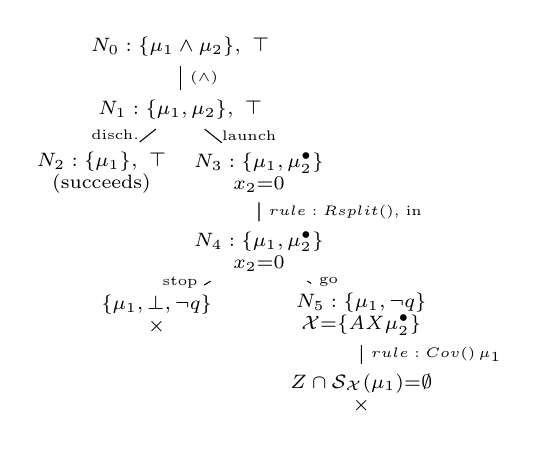
\begin{tikzpicture}[
  every node/.style={align=center, font=\scriptsize},
  level 1/.style={level distance=8mm},
  level 2/.style={sibling distance=20mm, level distance=8mm},
  level 3/.style={level distance=10mm},
  level 4/.style={sibling distance=26mm, level distance=8mm},
  level 5/.style={level distance=10mm},
  edge from parent/.style={draw,-}
]
\node {$N_0:\{\mu_1\wedge\mu_2\},\ \top$}
 child { node {$N_1:\{\mu_1,\mu_2\},\ \top$}
   child { node {$N_2:\{\mu_1\},\ \top$\\ (succeeds)}
     edge from parent node[left,font=\tiny,pos=.45]{disch.} }
   child { node {$N_3:\{\mu_1,\mu_2^\bullet\}$\\ $x_2{=}0$}
     child { node {$N_4:\{\mu_1,\mu_2^\bullet\}$\\ $x_2{=}0$}
       child { node {$\{\mu_1,\bot,\neg q\}$\\ $\CLOSED$}
         edge from parent node[left,font=\tiny,pos=.5]{stop} }
       child { node {$N_5:\{\mu_1,\neg q\}$\\ $\Ctx{=}\{\AX\mu_2^\bullet\}$}
         child { node {$Z\cap\Sat_\Ctx(\mu_1){=}\emptyset$\\ $\CLOSED$}
           edge from parent node[right,font=\tiny,pos=.5]{$\rlink{Cov}\,\mu_1$} }
         edge from parent node[right,font=\tiny,pos=.5]{go} }
       edge from parent node[right,font=\tiny]{$\rlink{Rsplit}$, in} }
     edge from parent node[right,font=\tiny,pos=.45]{launch} }
   edge from parent node[right,font=\tiny]{$(\wedge)$} };
\end{tikzpicture}}
\subcaption{$\mu_1\wedge\mu_2$: \UNSAT.}\label{fig:ex-unsat}
\end{subfigure}
\hfill
\begin{subfigure}[t]{0.49\textwidth}\centering
\resizebox{\linewidth}{!}{%
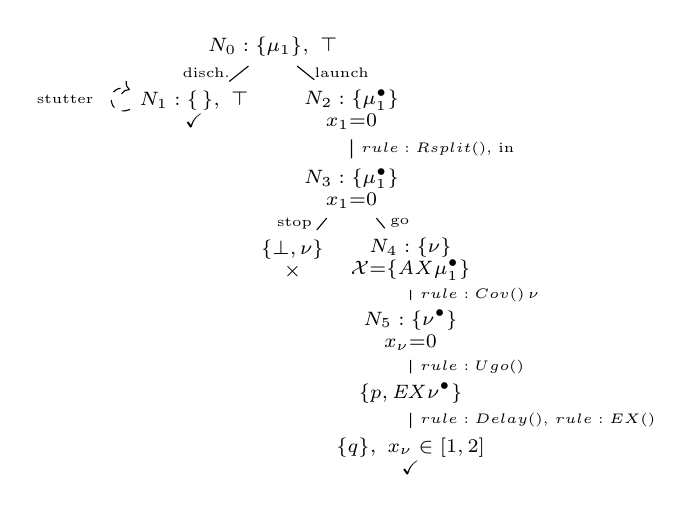
\begin{tikzpicture}[
  every node/.style={align=center, font=\scriptsize},
  level 1/.style={sibling distance=20mm, level distance=8mm},
  level 2/.style={level distance=10mm},
  level 3/.style={sibling distance=15mm, level distance=9mm},
  level 4/.style={sibling distance=20mm, level distance=9mm},
  level 5/.style={level distance=8mm},
  edge from parent/.style={draw,-}
]
\node {$N_0:\{\mu_1\},\ \top$}
 child { node (free) {$N_1:\{\,\},\ \top$\\ $\OPEN$}
   edge from parent node[left,font=\tiny,pos=.45]{disch.} }
 child { node {$N_2:\{\mu_1^\bullet\}$\\ $x_1{=}0$}
   child { node {$N_3:\{\mu_1^\bullet\}$\\ $x_1{=}0$}
     child { node {$\{\bot,\nu\}$\\ $\CLOSED$}
       edge from parent node[left,font=\tiny,pos=.5]{stop} }
     child { node {$N_4:\{\nu\}$\\ $\Ctx{=}\{\AX\mu_1^\bullet\}$}
       child { node {$N_5:\{\nu^\bullet\}$\\ $x_\nu{=}0$}
         child { node {$\{p,\EX\nu^\bullet\}$}
           child { node {$\{q\},\ x_\nu\in[1,2]$\\ $\OPEN$}
             edge from parent node[right,font=\tiny,pos=.5]{$\rlink{Delay}$, $\rlink{EX}$} }
           edge from parent node[right,font=\tiny,pos=.5]{$\rlink{Ugo}$} }
         edge from parent node[right,font=\tiny,pos=.5]{$\rlink{Cov}\,\nu$} }
       edge from parent node[right,font=\tiny,pos=.5]{go} }
     edge from parent node[right,font=\tiny]{$\rlink{Rsplit}$, in} }
   edge from parent node[right,font=\tiny,pos=.45]{launch} };
\draw[->,dashed] (free.west) to[out=200,in=160,looseness=3.4]
  node[left=3pt,font=\tiny]{stutter} ([yshift=-3pt]free.north west);
\end{tikzpicture}}
\subcaption{$\mu_1$ alone: \SAT.}\label{fig:ex-sat}
\end{subfigure}
\caption{Tableau runs, with $\nu=\tEU{p}{q}{[1,2]}$, $\mu_1=\mathrm{AG}_{[0,4]}\nu$,
$\mu_2=\mathrm{AG}_{[0,3]}\neg q$.}\label{fig:ex}
\end{figure}

\begin{example}[$\mu_1\wedge\mu_2$]\label{ex:unsat}
After $(\wedge)$, covering $\mu_2$ succeeds under the empty context and splits $N_1$
into a discharge child and a launch child $N_3$, which carries $\mu_1$ alongside the
pursuit. At $N_3$ the zone is the point $x_2{=}0$, so \ruleref{Rsplit} leaves only its
in-part; \ruleref{Runf_in} closes the stop child on $\bot$ and yields $N_5$, where the
context now forces $\neg q$ wherever $x_2\in[0,3]$.

Covering $\mu_1$ there fails. Computing $\Sat_\Ctx(\mu_1)$ unfolds it to a demand for
$\nu$ at the onset, and unfolding $\nu$ by \ruleref{Uunf} closes both branches:
\ruleref{Ustop} lands on $x_\nu\in[1,2]$, which coincides with $x_2\in[1,2]\subseteq[0,3]$,
so the node carries $q$ and $\neg q$; \ruleref{Ugo} defers with no deadline to cap it, and
once $x_\nu>2$ the window has passed with the stop never taken, so every repeat fails
acceptance condition~(i). Hence $\Sat_\Ctx(\nu)=\emptyset$ at this onset,
$Z\cap\Sat_\Ctx(\mu_1)=\emptyset$, and neither \ruleref{Cov} nor \ruleref{Covstar} applies:
$N_5$ closes and the formula is \UNSAT. The calculus never compares the two modalities
directly; it only brings $q$ and $\neg q$ into one goal set over overlapping zones.
\end{example}

\begin{example}[$\mu_1$ alone]\label{ex:sat}
Without $\mu_2$ nothing constrains $q$, so covering $\nu$ at $N_4$ succeeds and launches
its pursuit with $x_\nu$ reset. That pursuit shows how a window is entered: at $N_5$ the
zone is $x_\nu{=}0$, so \ruleref{Ustop} has empty zone and closes, and only \ruleref{Ugo}
survives, asserting $p$ and deferring $\EX\nu^\bullet$. The resulting node is saturated,
so \ruleref{Delay} advances the zone and \ruleref{EX} supplies the successor carrying
$\nu^\bullet$; at the first one with $x_\nu\in[1,2]$ the stop child is consistent and the
eventuality is fulfilled.

Meanwhile $\AX\mu_1^\bullet$ rides every successor, re-imposing $\mu_1$ across its window.
Once $x_1>4$ the after-part of \ruleref{Rsplit} drops $\mu_1^\bullet$, leaving a goal-free
node whose stutter loop is accepting: no until pursuit is active, so condition~(i) is
vacuous, and $x_1$ is extrapolated above $M{=}4$. The cycle can only live in this lapsed
tail, since inside the window the release's own split bounds $x_1$. The marking succeeds,
and reading it off gives a one-location automaton labelled $p$ with a $q$-successor
reachable within $[1,2]$ of each onset.
\end{example}


\section{The Tableau}\label{sec:tableau}
%
%
%We decide satisfiability of an input formula $\varphi$ by a depth-first, on-the-fly construction that
%builds a graph of symbolic nodes and searches it for a \emph{successful marking}. A node carries the
%formulas to be realised at a configuration, and zones represent clock valuations symbolically. A
%time-bounded modality is never tested against a precomputed set of valuations: it is discharged by
%\emph{pursuing} it, so that the search itself produces the witness. We fix nodes and realisability
%(\S\ref{ss:nodes}), give the rules (\S\ref{ss:rules}), define acceptance and its test
%(\S\ref{ss:loop}), and close with two examples (\S\ref{ss:ex}).
%
We decide satisfiability of $\varphi$ by an on-the-fly, symbolic tableau construction.
%
%A time-bounded modality is never tested against a precomputed set of valuations but discharged by
%\emph{pursuing} it, so that the search itself produces the witness. 
%
We fix nodes and realisability
(\S\ref{ss:nodes}), give the rules (\S\ref{ss:rules}), define acceptance (\S\ref{ss:loop}), and
close with two examples (\S\ref{ss:ex}).

\subsection{Nodes and Realisability}\label{ss:nodes}


A {node} is a tuple $N=\tup{\Gamma}{\Ctx}{Z}{\obligations}{\Deadline}$, where $\Gamma$ is the set of
goal formulas to be satisfied (write $\Gamma_{\mathsf{prop}}=\Gamma\cap\big(\mathcal P\cup\{\neg p\mid p\in\mathcal P\}\big)$ for the propositional part); $\Ctx$ the {context} of universal formulas that must
hold at every successor; $Z$ the set of clock valuations for this node, represented as a canonical zone; $\obligations$ the {clock map}, which allocates to every active timed modality $\mu$ a dedicated formula-clock $x_\mu$ so its window (i.e. its interval \kI) can be measured from the configuration that demanded it; and $\Deadline$ is a set of deadlines
$(x_\mu,\sup\kI)$, each with a strictness flag, and $\Inv(N)=\bigwedge_{(x_\mu,b)\in \Deadline}x_\mu\le b$
its induced invariant. Besides these five components a node records the clocks reset by the rule
that produced it and, if that rule was a stop branch, the modality it discharged; a rule sets both
from the branch it takes, and we leave them implicit in the displays below.

%%%%%%%%% DEAD TEXT %%%%%%%%
% $\equiv$ is defined again below, after realisability, and closedness both below
% and in \S\ref{ss:loop}.
%Two nodes are
%\emph{equivalent}, written $N\equiv N'$, when they agree in $\Gamma$, $\Ctx$, $\obligations$, $\Deadline$ and
%in these two records, and their zones agree modulo $\cong_M$. A node is \emph{closed} when
%$\Gamma_{\mathsf{prop}}$ contains a complementary pair $p,\neg p$ or its zone is empty. Closed
%nodes have no children.
%%%%%%%%% DEAD TEXT %%%%%%%%

%A deadline is added when \ruleref{Cov} launches the pursuit of a
%universal until and removed when the $(\text{stop})$ branch of \ruleref{Uunf} discharges it;
%no other rule writes $\Deadline$.
%
%; and $\eventualities$ the postponed eventualities used for loopacceptance. 


%Write $\Gamma_{\mathsf{prop}}=\Gamma\cap\big(\mathcal P\cup\{\neg p\mid p\in\mathcal P\}\big)$ for the {propositional part} of $\Gamma$, the atomic literals it asserts. A node is {closed} if $\Gamma_{\mathsf{prop}}$ is propositionally inconsistent, i.e., it contains a complementary pair $p,\neg p$ (equivalently $\bot\in\Gamma$), or its zone is empty, $Z=\emptyset$; it is {saturated} when no expansion rule applies.



%\noindent
%We write
%$\Gamma_{\mathsf{prop}}=\Gamma\cap\big(\mathcal P\cup\{\neg p\mid p\in\mathcal P\}\big)$ for the
%\emph{propositional part} of $\Gamma$, the atomic literals it asserts. 

%%%%%%%%% DEAD TEXT %%%%%%%%
% A path is defined again in \S\ref{ss:loop}, where the tableau graph is introduced
% and paths are first used.
%We call a sequence of nodes $N_0,N_1,\dots$ a \emph{path} if each $N_{i+1}$ is a child of $N_i$.
%%%%%%%%% DEAD TEXT %%%%%%%%

%Write
%\[
%  \Inv(N)\hspace{-0.1cm}=\hspace{-0.1cm}\bigwedge\big\{x_\mu\le\sup\kI \big| \mu=\mathrm{A}(\varphi\mathbf{U}_\kI\psi)
%  \text{ under pursuit at } N \big\} \quad (<\text{ if } \sup\kI\notin\kI)
%\]
%for the node's {invariant}. Both $x_\mu$ and the bound are read off the node: the clock
%from $\obligations$, the interval from $\mu$ itself.
%
%$\clocks(\obligations)$
A node is \emph{closed} if its zone is empty, $Z=\emptyset$, since it then has no valuations to
realise, or if $\bot\in\Gamma_{\mathsf{prop}}$. It is
\emph{saturated} when no saturation or cover rule applies; only saturated nodes generate successors.
It is \emph{realisable} if there is a non-blocking TTS $\mathcal T$ induced by a TA, a location $s$ with
$L(s)\supseteq\Gamma_{\mathsf{prop}}$ and $\Inv(s)=\Inv(N)$, and an interpretation of the
formula-clocks in \obligations, such that for every $\nu \in Z$ the configuration $(s,\nu)$  $\mathcal T,(s,\nu)\models\textstyle\bigwedge\Gamma\ \wedge\ \bigwedge\Ctx$. 
Realisability is {monotone under narrowing}: if $\tup{\Gamma}{\Ctx}{Z}{\obligations}{\Deadline}$ is realisable and
$\emptyset\neq Z'\subseteq Z$, then so is $\tup{\Gamma}{\Ctx}{Z'}{\obligations}{\Deadline}$.


%Two consequences of Definition~\ref{def:realisable} shape the calculus. First, the quantification over $Z$ is \emph{universal}: this is precisely what lets a single node discharge a demand re-imposed by a persistent context at a continuum of onsets. Second, realisability is \emph{monotone under narrowing}.

%\begin{lemma}[Narrowing]\label{lem:narrowing}
%If $\tup{\Gamma}{\Ctx}{Z}{\obligations}$ is realisable and
%$\emptyset\neq Z'\subseteq Z$, then $\tup{\Gamma}{\Ctx}{Z'}{\obligations}$ is realisable.
%\end{lemma}
%\begin{proof}
%Immediate: the condition of Definition~\ref{def:realisable} is universally quantified over the zone, and
%$Z'$ is a non-empty subset of $Z$.
%\end{proof}
%
%Lemma~\ref{lem:narrowing} is what licenses the refinement rule \ruleref{Covstar} to be a disjunctive
%choice rather than a case analysis: a node is free to commit to a tighter entry constraint. For this to
%be sound at the level of the extracted automaton, the narrowing must happen \emph{before} the node's
%outgoing steps are fixed; this is guaranteed by the discipline of \S\ref{ss:rules}, where a node is
%saturated and covered to exhaustion before any successor is generated, so the guards of its delays and
%edges are read off the narrowed zone.

%\noindent

Two nodes $N_1$ and $N_2$ are \emph{equivalent}, written $N_1\equiv N_2$, when they agree in $\Gamma$, $\Ctx$, $\obligations$, $\Deadline$, in the
clocks reset by the rule that produced them and in the modality that rule discharged, and their
zones agree modulo $\cong_M$.


An \emph{OR} (disjunctive, $\ORn$) node is realisable if
\emph{some} child is; an \emph{AND} (conjunctive, $\ANDn$) node requires \emph{all} its children. Some
rules are deterministic ($\DETn$): a single child, replacing the node.  We write $kind(N)\in\{\DETn,\ORn,\ANDn\}$.





%Table~\ref{tab:rulekinds} fixes the kind of every rule; the marginal marker on each rule below repeats it.

%\begin{table}[t]
%\centering
%\caption{Every rule and its branching kind. $\DETn$ = single child, $\ORn$ = OR-node,
%$\ANDn$ = AND-node.}\label{tab:rulekinds}
%\begin{tabular}{llll}
%\hline
%Group & Rule & Kind & Children \\
%\hline
%Saturation & $(\wedge)$, \ruleref{AX} & $\DETn$ & $1$ \\
%Saturation & $(\vee)$ & $\ORn$ & $2$ \\
%Cover & \ruleref{Cov} & $\ANDn$ & $2$ (discharge, launch) \\
%Cover & \ruleref{Covstar} & $\ORn$ & one per convex component \\
%Pursuit & \ruleref{Uunf} & $\ORn$ & $2$ (stop, go) \\
%Pursuit & \ruleref{Rsplit} & $\ANDn$ & $\le 3$ (before, in, after) \\
%Pursuit & \ruleref{Runf} & $\ORn$ & $2$ per part \\
%Successors & \ruleref{Delay} & $\ANDn$ & $2$ (open segment, boundary) \\
%Successors & \ruleref{EX} & $\ANDn$ & one per $\EX\psi\in\Gamma$, or stutter \\
%\hline
%\end{tabular}
%\end{table}
%
\noindent


%A \emph{marking} $\mathcal M$ selects one child at each OR-node and \emph{all} children at each
%AND-node; it is \emph{successful} if it contains no closed node and every postponed eventuality is
%fulfilled on every infinite path, in the sense made effective by the loop condition of
%\S\ref{ss:loop}. 



%The tableau \emph{succeeds} on $\varphi$ if the root
%$\tup{\{\varphi\}}{\emptyset}{\Zuniv}{\emptyset}{\emptyset}$ admits a successful marking, where
%$\Zuniv$ is the universal zone over $\clockSet$.

\subsection{Rules}\label{ss:rules}
Rules come in four groups: \emph{saturation} decomposes goals, \emph{cover} discharges and
launches a timed modality, \emph{pursuit} unfolds a launched one step by step, and
\emph{successor generation} expands a saturated node.
%Each rule rewrites a node into its children, shown on the full tuple; a component reappears unchanged unless the rule modifies it.
%
%We consider four groups of rules: \emph{saturation} decomposes the goals in $\Gamma$, the \emph{cover} rule discharges a timed modality, the \emph{pursuit} rules unfold a launched modality one step at a time, and \emph{successor generation} expands a saturated node in time and across edges.
%%
%%Rules come in four groups: \emph{saturation}
%%decomposes the goals in $\Gamma$, the \emph{cover} rule discharges a timed modality, the
%\emph{pursuit} rules unfold a launched modality one step at a time, and \emph{successor
%generation} expands a saturated node in time and across edges.
%
\vspace{-0.1cm}
\paragraph{Saturation.}
Conjunction \ruleref{Conj} is deterministic, disjunction \ruleref{Disj} branches, and \ruleref{AX} handles a universal marker by moving its argument into the context. %There is no saturation rule for $\EX$: ``some successor satisfies
%$\psi$'' cannot be settled before successors exist, so $\EX\psi$ waits in $\Gamma$ and is discharged by
%\ruleref{EX}.
\vspace{-0.1cm}
\[
\footnotesize
\ \frac{\tup{\Gamma\cup\{\varphi\land\psi\}}{\Ctx}{Z}{\obligations}{\Deadline}}
{\tup{\Gamma\cup\{\varphi,\psi\}}{\Ctx}{Z}{\obligations}{\Deadline}}\quad
\shortstack{\ruleanchor{Conj}\\\DETn}
\qquad
\ \frac{\tup{\Gamma\cup\{\AX\varphi\}}{\Ctx}{Z}{\obligations}{\Deadline}}
{\tup{\Gamma}{\Ctx\cup\{\varphi\}}{Z}{\obligations}{\Deadline}}\quad
\shortstack{\ruleanchor{AX}\\ \DETn}
\]\vspace{-0.2cm}
\[
\footnotesize
\frac{\tup{\Gamma\cup\{\varphi\lor\psi\}}{\Ctx}{Z}{\obligations}{\Deadline}}
{
\begin{array}{ll}
\tup{\Gamma\cup\{\varphi\}}{\Ctx}{Z}{\obligations}{\Deadline}\\
  \tup{\Gamma\cup\{\psi\}}{\Ctx}{Z}{\obligations}{\Deadline}
\end{array}
}
%
%\ \frac{\tup{\Gamma\cup\{\varphi\lor\psi\}}{\Ctx}{Z}{\obligations}{\Deadline}}
%{\tup{\Gamma\cup\{\varphi\}}{\Ctx}{Z}{\obligations}{\Deadline}\quad\big|\quad
%\tup{\Gamma\cup\{\psi\}}{\Ctx}{Z}{\obligations}{\Deadline}}
\quad
\shortstack{\ruleanchor{Disj}\\\ORn
}
\]

\paragraph{Pursuing time modalities.}

When $\Gamma$ contains a timed modality $\mu=\mathrm{Q}(\varphi\circ_\kI\psi)$, with
$\mathrm{Q}\in\{\mathrm{E},\mathrm{A}\}$ and $\circ\in\{\mathbf{U},\mathbf{R}\}$, we say the node
\emph{demands} $\mu$, and $\mu$ must hold at every valuation of the node's zone. To fulfil the demand the rule produces a \ruleref{discharge} child, which drops $\mu$ from
$\Gamma$ and lets the node continue with its remaining goals, and a \ruleref{launch} child, which
starts a \emph{pursuit} of $\mu$, written $\mu^\bullet$, i.e., a branch that unfolds $\mu$ step by
step in search of a witness. The launch introduces a fresh formula-clock $x_\mu$ and resets it
here, so that $\kI$ is measured from this configuration.

\vspace{-0.3cm}
\[
\footnotesize
\frac{\tup{\Gamma\cup\{\mu\}}{\Ctx}{Z}{\obligations}{\Deadline}}
{\begin{array}{ll}
\tup{\Gamma}{\Ctx}{Z}{\obligations}{\Deadline} & \ruleanchor{discharge}\\[3pt]
\tup{\Gamma\cup\{\mu^\bullet\}}{\Ctx}{\rst{Z}{x_\mu}}{\obligations[\mu\mapsto x_\mu]}{\Deadline\cup \Deadline_\mu}
 & \ruleanchor{launch}
\end{array}}
\raisebox{-4ex}{
  \shortstack{
    $\obligations(\mu)$ undefined, or\\
    $\sup\kI<\infty$ and $\mu$ not\\
    a universal until}
}
\shortstack{\ruleanchor{Cov}\\\ANDn}
\]


%The rule is conjunctive because its children carry different work for one and the same
%configuration: the launches are what \emph{establish} $\mu$, one onset each, and the discharge is
%what lets the rest of $\Gamma$ be established alongside them. They are not alternatives, and none
%may be dropped. In particular the cross-product of the branches over several demands is what
%forces every demand of a node into a common leaf, where a contradiction between them closes it.
%
A deadline $\Deadline_\mu=\{(x_\mu,\sup\kI)\}$ is applied iff $\mu$ is a universal until, with
$\Deadline_\mu=\emptyset$ otherwise. Only such a modality needs one, as it obliges \emph{every} run to
satisfy $\psi$ within $\kI$ and time must be forced forward or a run could idle past the window with
the eventuality unmet. An existential until is discharged by a single witnessing run, and a release,
of either quantifier, is discharged by lapsing past the window rather than by acting within it.

%
%The side condition fires \ruleref{Cov} on a modality not yet under pursuit, and on one already
%pursued when its window is finite and it is not a universal until.
%

%A window with
%$\sup\kI=\infty$ leaves no bound to carry either way, and there the eventuality is forced instead by
%the acceptance condition on markings (\S\ref{ss:loop}).
%
%What that sharing costs is settledwhere the pursuit succeeds.

%Because the demand is discharged by construction, the calculus never has to narrow a node to the
%part of its zone on which $\mu$ happens to hold. Narrowing survives
%only where a rule genuinely partitions the zone, in \ruleref{Rsplit} and \ruleref{Delay} below, and
%it is there that monotonicity of realisability under narrowing is used.

\paragraph{Pursuing an Until.}





Consider an until modality $\mu=\mathrm{Q}(\varphi\mathbf{U}_\kI\psi)$, writing
$a=\inf\kI$ and $b=\sup\kI$. An ordinary pursuit $\mu^\bullet$ unfolds by \ruleref{Uunf}: either
$\psi$ holds now, inside the window, or $\varphi$ holds now and the pursuit passes to the
successors.
%
%
%Its unfolding is a disjunction: either $\psi$ holds now and the
%eventuality is met, which is the \ruleref{Ustop} branch, or $\varphi$ holds now and the pursuit is
%deferred to the successors, which is \ruleref{Ugo}. We call a pursuit \emph{persistent} once
%\ruleref{Carry} has folded a re-demand into it; for such a pursuit the stop branch takes a different
%form. 
\vspace{-0.1cm}
\[
\footnotesize
\frac{\tup{\Gamma\cup\{\mu^\bullet\}}{\Ctx}{Z}{\obligations}{\Deadline}}
{\begin{array}{ll}
\tup{\Gamma\cup\{\psi\}}{\Ctx}{Z\cap(x_\mu\in\kI)}{\obligations}{\Deadline\setminus\{(x_\mu,b)\}}
  & \ruleanchor{Ustop}\\[4pt]
\left\{
\begin{array}{ll}
\tup{\Gamma\cup\{\varphi,\EX\mu^\bullet\}}{\Ctx}{Z}{\obligations}{\Deadline}
  & \text{if } \mathrm{Q}=\mathrm{E},\\[3pt]
\tup{\Gamma\cup\{\varphi\}}{\Ctx\cup\{\AX\mu^\bullet\}}{Z}{\obligations}{\Deadline}
  & \text{if } \mathrm{Q}=\mathrm{A},
\end{array}
\right.
& \ruleanchor{Ugo}
\end{array}}
\shortstack{
$\mu=\mathrm{Q}(\varphi\mathbf{U}_\kI\psi)$}
\shortstack{\ruleanchor{Uunf}\\\ORn}
\]
\ruleref{Ugo} defers the pursuit to the successors, where $x_\mu$ keeps running and the window
stays open; for $\mathrm{Q}=\mathrm{E}$ a single witnessing run suffices, so the residual travels
as a goal to one successor, and for $\mathrm{Q}=\mathrm{A}$ every run must comply, so it travels
as context to all of them. \ruleref{Ustop} ends the pursuit: $\mu^\bullet$ is dropped from
$\Gamma$ and its deadline removed from $\Deadline$, the single onset it was launched for having
been answered.

Pursuit must end when the window closes, i.e., $x_\mu\in\kI$ fails. The rule \ruleref{Umiss} empties the zone and closes the node, which is then no longer realisable.
%
%Deferral ends with the window. The witness needs $x_\mu\in\kI$ and the clock only grows, so a
%zone lying wholly beyond a finite $b$ holds no moment for it; \ruleref{Umiss} empties the zone,
%and the node is closed.
\vspace{-0.2cm}
\[
\footnotesize
\frac{\tup{\Gamma\cup\{\mu^\bullet\}}{\Ctx}{Z}{\obligations}{\Deadline}}
     {\tup{\Gamma\cup\{\mu^\bullet\}}{\Ctx}{\emptyset}{\obligations}{\Deadline}}
\quad
\begin{array}{l}
%Z\cap(x_\mu\le b)=\emptyset,\\ b<\infty
x_\mu\not\in\kI, \\ b<\infty
\end{array}
\shortstack{\ruleanchor{Umiss}\\\DETn}
\]
For a universal until the deadline in
$\Deadline$ empties the zone first and the rule never fires.

%; for an existential until it settles
%the eventuality, \ruleref{Ugo} alone being available at every step. 
%%The rule carries no
%invariant: an existential demand is served by a single run, and an invariant binds them all.
%
\begin{figure}[t]
\centering
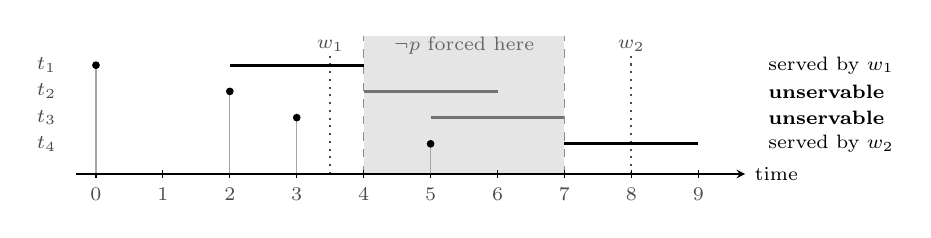
\begin{tikzpicture}[x=8.5mm,y=3.33mm,font=\scriptsize,>=stealth]

% band where p is forbidden
\fill[black!10] (4,-0.75) rectangle (7,4.5);
\draw[black!45,dashed] (4,-0.75) -- (4,4.5);
\draw[black!45,dashed] (7,-0.75) -- (7,4.5);
\node[black!60] at (5.5,4.15) {$\lnot p$ forced here};

% candidate times for p
\draw[black!70,dotted,thick] (3.5,-0.75) -- (3.5,3.9);
\node[black!70] at (3.5,4.15) {$w_1$};
\draw[black!70,dotted,thick] (8,-0.75) -- (8,3.9);
\node[black!70] at (8,4.15) {$w_2$};

% time axis
\draw[->] (-0.3,-0.75) -- (9.7,-0.75) node[right] {time};
\foreach \t in {0,1,2,3,4,5,6,7,8,9}
  \draw (\t,-0.9) -- (\t,-0.6) node[below=3pt,black!70] {$\t$};

% onset marks, named on the left
\foreach \o/\r/\lab in {0/3.4/{$t_1$}, 2/2.4/{$t_2$}, 3/1.4/{$t_3$}, 5/0.4/{$t_4$}} {
  \node[anchor=east,black!70] at (-0.45,\r) {\lab};
  \draw[black!35] (\o,\r) -- (\o,-0.7);
  \fill (\o,\r) circle (1.4pt);
}
% windows [t_i+2, t_i+4]
\draw[very thick] (2,3.4) -- (4,3.4);
\draw[very thick,black!55] (4,2.4) -- (6,2.4);
\draw[very thick,black!55] (5,1.4) -- (7,1.4);
\draw[very thick] (7,0.4) -- (9,0.4);

\node[anchor=west] at (9.9,3.4) {served by $w_1$};
\node[anchor=west] at (9.9,2.4) {\textbf{unservable}};
\node[anchor=west] at (9.9,1.4) {\textbf{unservable}};
\node[anchor=west] at (9.9,0.4) {served by $w_2$};

\end{tikzpicture}
\caption{The formula $\mathrm{AG}\,\mathrm{EF}_{[2,4]}\,p\wedge\mathrm{AG}_{[4,7]}\lnot p$ (\UNSAT). The bar at
$t_i$ is that onset's window $[t_i+2,t_i+4]$, and a $p$ at $w$ serves the onsets whose bar contains
it. The pursuit launched at $t_1$ stops at $w_1$ and serves no later onset.}\label{fig:onsets}
\end{figure}


As shown in Fig.~\ref{fig:onsets}, a demand can be potentially requested by a continuum of onsets. We handle it symbolically, according to whether $\sup I < \infty$ or not. 

\noindent
For $\sup I=\infty$, the new onset is absorbed into the running one: \ruleref{Absorb} drops
$\mu$ from $\Gamma$, so it is not demanded again, and keeps the previous pursuit alive. A new
one is launched only when the previous pursuit stops, so a run carries a stream of witnesses,
and every onset here asks only for a $\psi$ at some later point, which the stream supplies. 

\noindent
For $\sup I<\infty$, some onsets can not be absorbed, as shown in Fig.~\ref{fig:onsets}. In this case, we distinguish between the existential until, which is simply pursued by a new \ruleref{Cov}, and a universal until, which is \emph{carried}. Every run must comply with the demand, so one pursuit that witnesses at least every $b-a$ covers every onset and it turns \emph{persistent}, written $\mu^{\ast}$, which is unfolded by \ruleref{Uunfcarry}. 
\vspace{-0.2cm}
\[
\footnotesize
\frac{\tup{\Gamma\cup\{\mu,\mu^\bullet\}}{\Ctx}{Z}{\obligations}{\Deadline}}
     {\tup{\Gamma\cup\{\mu^{\ast}\}}{\Ctx}{Z}{\obligations}{\Deadline}}
  \hspace{-0.25cm}
\shortstack{
%$\mu=\mathrm{A}(\varphi\mathbf{U}_\kI\psi),$\\
$\mu$ universal \\ until,\\
$b<\infty$
}
\hspace{-0.33cm}
\shortstack{\ruleanchor{Carry}\\\DETn}
\hspace{0.2cm}
\footnotesize
\frac{\tup{\Gamma\cup\{\mu,\mu^{\dagger}\}}{\Ctx}{Z}{\obligations}{\Deadline}}
     {\tup{\Gamma\cup\{\mu^{\dagger}\}}{\Ctx}{Z}{\obligations}{\Deadline}}
\hspace{-0.37cm}
\raisebox{0ex}{
\shortstack{
$\mu^{\dagger}\in\{\mu^{\bullet},\mu^{\ast}\},$\\
$b=\infty\ \text{or}$\\
$ \mu^{\dagger}=\mu^{\ast}$
}
}
\hspace{-0.4cm}
\shortstack{\ruleanchor{Absorb}\\\DETn}
\]
\vspace{-0.35cm}
\[
\footnotesize
\frac{\tup{\Gamma\cup\{\mu^{\ast}\}}{\Ctx}{Z}{\obligations}{\Deadline}}
{\begin{array}{ll}
\tup{\Gamma\cup\{\psi,\mu^{\ast}\}}{\Ctx}{\rst{Z\cap(x_\mu\in\kIrec)}{x_\mu}}{\obligations}
{\Deadline[x_\mu\mapsto b-a]}
  & \ruleanchor{Ustopcarry}\\[4pt]
\tup{\Gamma\cup\{\varphi\}}{\Ctx\cup\{\AX\mu^{\ast}\}}{Z}{\obligations}{\Deadline}
  & \ruleanchor{Ugocarry}
\end{array}}
\hspace{-0.1cm}
\raisebox{-3ex}{
\shortstack{
$ b<\infty$\\
$\mu=\mathrm{A}(\varphi\mathbf{U}_\kI\psi)$
}
}
\hspace{-0.5cm}
\shortstack{\ruleanchor{Uunfcarry}\\\ORn}
\]
\ruleref{Ustopcarry} keeps the pursuit alive. A persistent pursuit answers every onset carried
into it, and the context keeps raising more, so $\mu^{\ast}$ stays and its clock restarts:
$x_\mu$ is re-zeroed, measuring from this occurrence of $\psi$, and its deadline is set to
$b-a$. That bound is the length of the window. A time $w$ at which $\psi$ holds answers exactly the
onsets in $[w-b,w-a]$, so two consecutive such times leave no onset unanswered precisely when
they lie within $b-a$ of each other. The guard follows the same reading: $\kIrec$ is \kI\ at the
first witness, where $x_\mu$ still measures from the onset that launched the pursuit, and $[0,b-a]$
at every later one, where it measures from the preceding witness. 

%Reading \kI\ throughout would ask
%consecutive witnesses to be at least $a$ apart while $\Deadline$ caps them at $b-a$, and for
%$2a>b$ no witness could follow the first.

%Take $\tAU{\top}{q}{[1,4]}$ demanded at every configuration. Witnesses four apart, at $0,4,8,\dots$,
%will not do: the onset at $3.5$ needs a $q$ in $[4.5,7.5]$, and the witness at $4$ is too early while
%the one at $8$ is too late. Witnesses three apart, at $0,3,6,\dots$, do: every window $[t+1,t+4]$ has
%length three, and points spaced three apart meet every interval of that length. The lower endpoint
%only shifts the window along the timeline; its length, $b-a$, is what fixes the rate. Read from the
%witness rather than the window, the same bound says that the oldest onset a witness at $w$ leaves
%unanswered lies just past $w-a$, has already waited $a$, and so runs out at $w+(b-a)$.
%%
%Where $b=\infty$ the bound is vacuous, every onset up to $w-a$ being answered at $w$, and all that
%survives of the requirement is that such times keep occurring. That is an eventuality with no
%deadline, which no invariant can bound and the acceptance condition on markings
%(\S\ref{ss:loop}) carries instead, so \ruleref{Carry} asks for a finite window.
%
%

%%%% Maybe adding it in the loop part later
%For $\mathrm{Q}=\mathrm{E}$
%no cap is needed, because $\mu$ was placed in $\eventualities$ at launch and a run that defers forever
%yields a non-fulfilling loop, rejected by \S\ref{ss:loop}; adding the cap there would only prune, never
%change the verdict.
%

\paragraph{Pursuing a Release.}
Consider now a release modality $\mu=\mathrm{Q}(\varphi\mathbf{R}_\kI\psi)$. The semantics of release imposes that $\psi$ must hold at every point in the window, unless $\varphi$ releases it. We handle the pursuit of a release in two stages. First, we partition the zone according to the position of $x_\mu$ relative to $\kI$, and then we pursue each part separately. We write $\ZltI = Z\cap(x_\mu<\inf\kI$ or $ x_\mu=\inf\kI\notin\kI)$, $\ZinI = Z\cap(x_\mu\in\kI)$ and $\ZgtI = Z\cap(x_\mu>\sup\kI$ or $ x_\mu=\sup\kI\notin\kI)$ for the three parts of the partition,
%
%
%\begin{align*}
%    \ZltI = Z&\cap(x_\mu<\inf\kI\ \text{or}\ x_\mu=\inf\kI\notin\kI),\quad \ZinI = Z\cap(x_\mu\in\kI),\quad\\
%    &\ZgtI = Z\cap(x_\mu>\sup\kI\ \text{or}\ x_\mu=\sup\kI\notin\kI),
%\end{align*}
%
so that the strictness of the interval endpoints is carried by the DBM bounds and the three parts are a partition of $Z$. Empty parts are dropped. Accordingly, the unfolding of a release produces up to three children, one for each part of the partition. The first two are pursued, while the last is lapsed and drops $\mu^\bullet$.
\vspace{-0.2cm}
\[
\footnotesize
\frac{\tup{\Gamma\cup\{\mu^\bullet\}}{\Ctx}{Z}{\obligations}{\Deadline}}
{\begin{array}{lll}
\tup{\Gamma\cup\{\mu^\bullet\}}{\Ctx}{\ZltI}{\obligations}{\Deadline} & \ruleanchor{Rsplitbefore}\\[2pt]
\tup{\Gamma\cup\{\mu^\bullet\}}{\Ctx}{\ZinI}{\obligations}{\Deadline} & \ruleanchor{Rsplitin}\\[2pt]
\tup{\Gamma}{\Ctx}{\ZgtI}{\obligations}{\Deadline} & \ruleanchor{Rsplitafter}
\end{array}}
\quad \mu=\mathrm{Q}(\varphi\mathbf{R}_\kI\psi)
\shortstack{\ruleanchor{Rsplit}\\\ANDn}
\]

The \ruleref{Rsplitbefore} and \ruleref{Rsplitin} parts are pursued by the following rule, which, similarly to \ruleref{Uunf} is a disjunction between two cases: either $\varphi$ is released, or the pursuit continues. %The \ruleref{Rsplitafter} part is lapsed and drops $\mu^\bullet$.
%Within the before and in parts the pursuit then either discharges through $\varphi$ or continues; this is a choice, hence an OR-node.
\vspace{-0.2cm}
\[
\footnotesize
\frac{\tup{\Gamma\cup\{\mu^\bullet\}}{\Ctx}{Z}{\obligations}{\Deadline}}
{\begin{array}{ll}
\tup{\Gamma\cup\Theta\cup\{\varphi\}}{\Ctx}{Z}{\obligations}{\Deadline} & \ruleanchor{Rstop}\\[3pt]
\left\{
\begin{array}{ll}
\tup{\Gamma\cup\Theta\cup\{\EX\mu^\bullet\}}{\Ctx}{Z}{\obligations}{\Deadline} & \text{if } \mathrm{Q}=\mathrm{E},\\[2pt]
\tup{\Gamma\cup\Theta}{\Ctx\cup\{\AX\mu^\bullet\}}{Z}{\obligations}{\Deadline} & \text{if } \mathrm{Q}=\mathrm{A},
\end{array}
\right.
& \ruleanchor{Rgo}
\end{array}}
\raisebox{-2ex}{\shortstack{$Z\subseteq\ZltI$ and $\Theta=\emptyset$,\\
or $Z\subseteq\ZinI$ and $\Theta=\{\psi\}$}}
\shortstack{\ruleanchor{Runf}\\\ORn}
\]



%\ruleref{Rstop} settles the demand at once and drops $\mu^\bullet$, while \ruleref{Rgo} defers it
%as \ruleref{Ugo} does.



\paragraph{Successor generation.}
A saturated and covered node is expanded by two successor rules.%, one elapsing time and one taking discrete steps.
%\emph{Both are AND-rules}: a model must admit the passage of time \emph{and} supply every demanded edge.
%The choice between waiting and moving is not made here --- it is made by the \ruleref{Ustop}/\ruleref{Ugo} branching of \ruleref{Uunf} and the corresponding 
%\ruleref{Runf_before}/\ruleref{Runf_in} branching of \ruleref{Runf}, which is where the existential content of the calculus lives.
\ruleref{Delay} advances the zone to the next integer hyperplane $x=b$ ($b\le M$) of an active bound,
and does so in two steps: $\Dopen Z$ is the time-successor of $Z$ strictly below the next
hyperplane, and $\Dbd Z$ is that hyperplane (equivalently $\uparrow Z$ when no hyperplane remains at or
below $M$). The hyperplanes of $x_\mu$ are the endpoints of $\kI$ together with their
\emph{shifts} $\inf\kI-\inf\kJ$ and $\sup\kI-\sup\kJ$ by the window \kJ\ of every other modality of
$\varphi$. The shifts are what keep onsets apart: a $\mu$ banning $\psi$ over $\kI$ leaves a demand
for $\psi$ over $\kJ$ unsatisfiable exactly at the onsets in $[\inf\kI-\inf\kJ,\sup\kI-\sup\kJ]$, and
splitting $x_\mu$ at the endpoints of \kI\ alone leaves that interval inside a cell that also holds
satisfiable onsets, whose witness then discharges the whole cell. There are two shifts per pair of
modalities and none depends on the magnitude of a constant, so the count of hyperplanes stays
quadratic in $|\varphi|$ and flat in $M$. %Both are computed under the node's invariant, which is where $\Inv(N)$ bounds the elapse:
\vspace{-0.2cm}
\[
\footnotesize
 \frac{\tup{\Gamma}{\Ctx}{Z}{\obligations}{\Deadline}}
{\begin{array}{ll}
\tup{\Gamma}{\Ctx}{\Dopen Z\cap\Inv(N)}{\obligations}{\Deadline} & \ruleanchor{openseg}\\[2pt]
\tup{\Gamma}{\Ctx}{\Dbd Z\cap\Inv(N)}{\obligations}{\Deadline} & \ruleanchor{boundary}
\end{array}}
\quad  \shortstack{$\Gamma$ \text{ saturated }\\ \text { and covered}}
\shortstack{\ruleanchor{Delay}\\ \ANDn }
\]

The two children carry the same demands and differ only in their zone, and that difference is
what a guard is tested against. Take a pursuit of $\mathrm{E}(p\mathbf{U}_{[1,2)}q)$ on the
zone $x_\mu\in(1,2)$, with $x_\mu=2$ the next hyperplane. On \ruleref{openseg} the
\ruleref{Ustop} guard $x_\mu\in[1,2)$ is non-empty, so $q$ may still be witnessed; on \ruleref{boundary} it is empty, the window having closed, and only \ruleref{Ugo} survives with an
eventuality that can no longer be met. A single zone spanning both would have to answer once
for two regions, and $[1,2)$ would become indistinguishable from $[1,2]$. Splitting keeps them
apart at no cost in the extracted automaton, where a chain of delay steps is one continuous
elapse within a single location.

%The goals are carried unchanged across a delay: a delay does not change location, and the pursuit residuals in $\Gamma$ are obligations of the run, not of a single configuration, so they must survive it.
%Saturation is re-run at each delay successor, since the narrowed zone may newly satisfy or falsify a guard.

\ruleref{EX} takes the discrete steps and discharges the existential markers, one child per demanded
$\EX\psi$, each carrying $\psi$ under the full context:
\vspace{-0.2cm}
\[
\footnotesize
\ \frac{\tup{\Gamma}{\Ctx}{Z}{\obligations}{\Deadline}}
{\big(\ \tup{\{\psi\}\cup\Ctx}{\Ctx}{Z}{\obligations}{\Deadline}\ \big)_{\EX\psi\in\Gamma}}
\quad  \shortstack{$\Gamma$ \text{ saturated }\\ \text { and covered}}
\shortstack{\ruleanchor{EX}\\ \ANDn }
\]
When no $\EX\psi\in\Gamma$, a single \emph{stutter} child
$\tup{\Ctx}{\Ctx}{Z}{\obligations}{\Deadline}$ keeps the run alive. Each child inherits $\Ctx$, allowing \ruleref{AX} to take effect, and it is why universal obligations constrain the whole
branching rather than one path. A pursuit's residual rides both kinds of successor: $\EX\mu^\bullet$ in $\Gamma$ reaches one, $\AX\mu^\bullet$ in $\Ctx$ reaches all. So $x_\mu$ advances by elapsing time as well as across edges.
A timed window is therefore entered by delay, its in-window stop taken at the first successor that
satisfies it; a pure-delay witness, i.e., waiting in one location until $x_\mu\in\kI$, then stopping, is a
chain of time-successors ending in a stop, the stutter step supplying a discrete anchor only when the
location must be left.

%% Proposed replacement for \subsection{Acceptance} in sec/section4_nosat.tex.
%% Keeps the label ss:loop and the labels M1, M2; adds def:children, def:graph.
%% 
% \rlink expands to bare math; \rl is the text-mode-safe form used below.
\newcommand{\rl}[1]{\ensuremath{\rlink{#1}}}

\subsection{Two Worked Runs of The Tableau}\label{ss:ex}


Consider the formula $\mathrm{AG}\,\mu\wedge\mathrm{AG}(q\rightarrow\sigma)$ with $\mu=\tAU{\top}{q}{[1,4]}$, that is $\mathrm{AF}_{[1,4]}q$, and 
$\sigma=\tAR{\bot}{\neg q}{(0,3]}$, that is $\mathrm{AG}_{(0,3]}(\lnot q)$. The first conjunct demands a $q$ within
$[1,4]$ of every configuration; the second forbids a $q$ for $3$ time units after each one. The left conjunct proceeds as a persistent demand. Its first demand launches $\mu^\bullet$ with $x$
reset and the deadline $x\le\sup\kI=4$; the next re-demand meets a live pursuit, so \ruleref{Carry}
folds it in and the pursuit becomes $\mu^{\ast}$. Meanwhile the right conjunct re-imposes its body
$\neg q\vee\sigma$ at every configuration, so $N_2$ carries both, and the disjunction is settled
before $\mu^{\ast}$ is unfolded.
\noindent
Take $\neg q$, at $N_3$. The pursuit can then neither take \ruleref{Ustopcarry} nor \ruleref{Ugocarry}: \ruleref{Ustopcarry} would assert
$q$ into a goal set already holding $\neg q$, and \ruleref{Ugocarry} can only defer, which past $x=4$
empties the zone against the deadline. Both children close.
\noindent
Take $\sigma$ instead. It is launched with its own clock $z$ reset, and \ruleref{Ustopcarry} asserts
$q$, re-zeroing $x$ and recapping it at $b-a=3$; this is $N_4$, where the two clocks begin to run
together, $x=z$. That is the contradiction. The carried deadline $x\le3$ says the next $q$ is due
within $3$, while $\sigma$ forbids $q$ for as long as $z\in(0,3]$. At $N_5$ the \ruleref{Ustopcarry} branch needs a
$q$ it cannot have, and \ruleref{Ugocarry} needs $x>3$, which the deadline denies. Both children close,
so $N_2$ closes and the formula is \UNSAT.

\input{figs/example}

%\begin{example}%[A Zeno cycle that may be left]\label{ex:zeno}
Consider $\mathrm{EG}_{[1,5]}\,\nu$, where $\nu=\tEU{\top}{p}{[2,4]}$. Write $x$ for the clock of
the release, and $y$ for that of $\nu$. \ruleref{Cov} splits $N_0$ into a discharge child, which
carries no pursuit, and the launch $N_2$, where $x$ is reset. \ruleref{Rsplit} then partitions the zone,
conjunctively, into its three parts. At $N_3$, the \ruleref{Rsplitbefore} part, \ruleref{Delay} carries $x$ into  \kI. $N_8$, where $x>5$, drops $\mu^\bullet$ and leaves a goal-free node that
may delay indefinitely: a time-progressing loop, since no until needs to be fulfilled and $x$ is
extrapolated above $M$.
\noindent
$N_4$ represents the \ruleref{Rsplitin} part of \ruleref{Rsplit}, where $\nu$ is inserted into $\Gamma$ and so
demanded. \ruleref{Cov} applies, giving two conjunctive branches. The \ruleref{launch} child $N_6$
proves $\nu$. It carries $\nu^\bullet$ with $y$ reset; its \ruleref{Ustop} is empty there, the window
$[2,4]$ not yet open, so only \ruleref{Ugo} survives until a delay carries $y$ into $[2,4]$, where
\ruleref{Ustop} asserts $p$ and drops $\nu^\bullet$. The \ruleref{discharge} child $N_5$ drops $\nu$
from $\Gamma$ and carries $\mu^\bullet$ on; a delay and \ruleref{EX} revive the release, still inside
$[1,5]$, and its in-part demands $\nu$ once more. The search is back at $N_4$, closing a loop. That
loop is not time-progressing: $x$ is never reset, and the in-window zone holds it below $5$.
\noindent
Nonetheless, we can construct a successful marking  as $\mathcal M=\{N_0,\allowbreak N_1,\allowbreak N_2,\allowbreak N_3,\allowbreak N_4,\allowbreak N_5,\allowbreak N_6,\allowbreak N_7,\allowbreak N_8\}$. \ref{M2} holds because the only until pursuit is $\nu^\bullet$, active at $N_6$, and the path to
$N_7$ takes its \ruleref{Ustop} at a node whose zone meets $y\in[2,4]$. \ref{M1} holds because every node of
$\mathcal M$ reaches a time-progressing loop: the nodes carrying the release reach $N_8$ by delaying
until $x$ passes $5$, which lapses it, while $N_1$ and, once $\nu^\bullet$ is dropped, $N_7$ carry
no pursuit, so no deadline caps their delays and their stutter loops are time-progressing. So $\mathcal M$, as well as the tableau, are successful and
$\mathrm{EG}_{[1,5]}\,\nu$ is \SAT.
 still follows it.

\subsection{The Tableau Graph and Acceptance}\label{ss:loop}

Through application of the rules, the tableau builds a graph of nodes, which can be used to establish satisfiability. 




To build this graph we settle which rule fires at a node, since rule application is
non-deterministic: several rules may apply to a node, which inherits the kind of the rule fired at it, and
one rule may apply to several goals.
Writing $\Subt(\varphi)$ for the timed modalities of $\FL(\varphi)$ and
$P=\FL(\varphi)\cup\{\mu^\bullet,\mu^{\ast}\mid\mu\in\Subt(\varphi)\}$, we define
$\FL^{\bullet}(\varphi)=P\cup\{\EX\chi,\AX\chi\mid\chi\in P\}$, with $|\FL^{\bullet}(\varphi)|=O(|\FL(\varphi)|)$. No rule produces a goal or a
context formula outside $\FL^{\bullet}(\varphi)$.



We fix, arbitrarily, a linear order \FormalSmaller{} on formulas (e.g., lexicographic)
and fire on the \FormalSmaller-least goal of $\Gamma$ to which a rule applies: a conjunction \ruleref{Conj}, a disjunction \ruleref{Disj}, an
$\AX\varphi$ \ruleref{AX}, a demanded modality \ruleref{Cov}, \ruleref{Carry} or \ruleref{Absorb}
as their side conditions prescribe, an until pursuit past a bounded window \ruleref{Umiss}, an
ordinary until pursuit $\mu^\bullet$ \ruleref{Uunf}
and a persistent one $\mu^{\ast}$ \ruleref{Uunfcarry}, and a release pursuit
\ruleref{Runf} when its zone lies wholly before or wholly inside
the window and \ruleref{Rsplit} otherwise.

This strategy produces for each node $N$ a set of children $\ch(N)$. A closed node has no children,
and the children of a saturated one are the \ruleref{Delay}- and the
\ruleref{EX}-children together, both successor rules being conjunctive, so it is an \ANDn-node.





The tableau graph $\TabGraph = (\TabNode, \TabEdge)$ is then constructed from the nodes reachable under $\ch$ from the
root $N_0=\tup{\{\varphi\}}{\emptyset}{\{\mathbf 0\}}{\emptyset}{\emptyset}$: its vertices $V$ are
those nodes up to $\equiv$, and it has an edge $e\in E$ from $N$ to every $N'\in\ch(N)$. A \emph{path} of $\TabGraph$ is a sequence of vertices, each a child of the preceding one, and a \emph{cycle} is a path returning to its first vertex.


\begin{lemma}%[Finiteness]
  \label{lem:finiteness}
$|\TabNode|\le 2^{O(n)}\cdot M^{O(n^{2})}$, and every node has $O(n)$ children.
\end{lemma}
\begin{proof}
  Each component of a node ranges over a set of size $2^{O(n)}$: $\Gamma$ and $\Ctx$ over subsets
of $\FL^{\bullet}(\varphi)$; $\obligations$ over subsets of $\Subt(\varphi)$, being determined by
its domain; $\Deadline$ over the assignments to each $x_\mu$ of $\sup\kI$ or $\sup\kI-\inf\kI$ with a
strictness flag; the reset set over subsets of $\clockSet$; and the discharged modality over
$\Subt(\varphi)$. A $\cong_M$-zone over $K\le n+1$ clocks is a $(K{+}1)^{2}$ DBM whose
entries are $\infty$ or lie in $\{-M,\dots,M\}\times\{<,\le\}$, so there are $M^{O(n^{2})}$ of
them. Thus the bound is $2^{O(n)}\cdot M^{O(n^{2})}$. Every rule has at most three children except
\ruleref{EX}, with one per $\EX\psi\in\Gamma$ and $|\Gamma|=O(n)$,.
\end{proof}


A \emph{marking} $\mathcal M \subseteq \TabNode$ is a set of vertices containing no closed node and containing, of each
of its members, at least one child if that node is an \ORn-node and all of them if it is an
\ANDn-node. A cycle of $\mathcal M$ is \emph{time-progressing} if it elapses positive time and every
clock is either reset on it or extrapolated above $M$. 

$\mathcal M$ is \emph{successful} if
every $N\in\mathcal M$ satisfies
\begin{enumerate*}[label={\textbf{(M\arabic*)}}, ref={\textbf{(M\arabic*)}},
                   itemjoin={{; }}, itemjoin*={{; and }}]
\item\label{M1} some path of $\mathcal M$ from $N$ meets a time-progressing cycle
\item\label{M2} for every until pursuit $\mu$ active at $N$,  some path of
$\mathcal M$ from $N$ that carries it throughout, with $x_\mu$ unreset along the way, takes a stop
branch (\ruleref{Ustop} or
\ruleref{Ustopcarry}) at a node $N_k$ with $Z_k\cap(x_\mu\in\kI)\neq\emptyset$.
\end{enumerate*}
\noindent
A tableau \emph{succeeds} on $\varphi$ if $N_0$ lies in a successful marking.


\ref{M2} ensures that an until pursuit is fulfilled rather
than deferred for ever through \ruleref{Ugo}. Its clause on $x_\mu$ ties the stop to the onset
the pursuit measures: a relaunch on the way restarts the clock, and a stop taken past it
witnesses the later onset.
\ref{M1} excludes Zeno witnesses. A clock never reset on a cycle and bounded there by some $k\le M$
caps the delays of all its traversals at $k$, so infinitely many traversals elapse only finitely much
time. The run they describe lies outside $\mathrm{Runs}^\infty$, on which satisfaction is defined,
and is a behaviour no system exhibits. The requirement that a cycle elapse positive time rules out
cycles built from expansion steps alone. Consider a persistent pursuit that has already carried over once: $\psi$ is a goal,
$x_\mu=0$, and the deadline on $x_\mu$ is $b-a$. If $0\in\kI$, a second application of
\ruleref{Ustopcarry} yields the same node, since the goal it adds is already present, the clock
it resets is already zero, and the deadline it sets is already in force. The node is its own
child, and the resulting self-loop elapses no time, so \ref{M1} keeps the node only if another
path leaves it.




%Both clauses read edges and not nodes: \ref{M1} inspects the clocks a cycle resets, \ref{M2} the
%branch on which a pursuit stops. This is why Definition~\ref{def:graph} compares the two records a
%node keeps of them. Without them a node reached through a reset and one reached without it would be
%merged, and a cycle through the merged node could report a reset that it never performs.
%

%
%Not every cycle of $\TabGraph$ crosses a successor step. \ruleref{Ustopcarry} re-imposes $\mu^{\ast}$
%on a node whose zone it has just reset, and for $\inf\kI=0$ the result can be the node it started
%from; Definition~\ref{def:graph} identifies the two, so a chain of rule applications that would
%regress for ever closes a cycle instead. Such a cycle elapses no time, so \ref{M1} discards it, and
%the calculus needs no separate argument that rule application terminates.
%
%Both clauses ask for reachability inside $\mathcal M$ rather than constraining every cycle
%separately, which is what the semantics calls for: TCTL quantifies over time-divergent runs, so what
%a witness owes at a reachable configuration is \emph{one} divergent continuation, not that every
%continuation diverge. Example~\ref{ex:zeno} exhibits a node whose only local cycle is Zeno and which
%belongs to a successful marking nonetheless.
%


% \rlink expands to bare math; \rl is the text-mode-safe form used below.
\newcommand{\rl}[1]{\ensuremath{\rlink{#1}}}

\subsection{Two Worked Runs of The Tableau}\label{ss:ex}


Consider the formula $\mathrm{AG}\,\mu\wedge\mathrm{AG}(q\rightarrow\sigma)$ with $\mu=\tAU{\top}{q}{[1,4]}$, that is $\mathrm{AF}_{[1,4]}q$, and 
$\sigma=\tAR{\bot}{\neg q}{(0,3]}$, that is $\mathrm{AG}_{(0,3]}(\lnot q)$. The first conjunct demands a $q$ within
$[1,4]$ of every configuration; the second forbids a $q$ for $3$ time units after each one. The left conjunct proceeds as a persistent demand. Its first demand launches $\mu^\bullet$ with $x$
reset and the deadline $x\le\sup\kI=4$; the next re-demand meets a live pursuit, so \ruleref{Carry}
folds it in and the pursuit becomes $\mu^{\ast}$. Meanwhile the right conjunct re-imposes its body
$\neg q\vee\sigma$ at every configuration, so $N_2$ carries both, and the disjunction is settled
before $\mu^{\ast}$ is unfolded.
\noindent
Take $\neg q$, at $N_3$. The pursuit can then neither take \ruleref{Ustopcarry} nor \ruleref{Ugocarry}: \ruleref{Ustopcarry} would assert
$q$ into a goal set already holding $\neg q$, and \ruleref{Ugocarry} can only defer, which past $x=4$
empties the zone against the deadline. Both children close.
\noindent
Take $\sigma$ instead. It is launched with its own clock $z$ reset, and \ruleref{Ustopcarry} asserts
$q$, re-zeroing $x$ and recapping it at $b-a=3$; this is $N_4$, where the two clocks begin to run
together, $x=z$. That is the contradiction. The carried deadline $x\le3$ says the next $q$ is due
within $3$, while $\sigma$ forbids $q$ for as long as $z\in(0,3]$. At $N_5$ the \ruleref{Ustopcarry} branch needs a
$q$ it cannot have, and \ruleref{Ugocarry} needs $x>3$, which the deadline denies. Both children close,
so $N_2$ closes and the formula is \UNSAT.


\begin{figure}[h]
\centering
\begin{subfigure}[b]{0.5\textwidth}\centering
\resizebox{0.8\linewidth}{!}{%
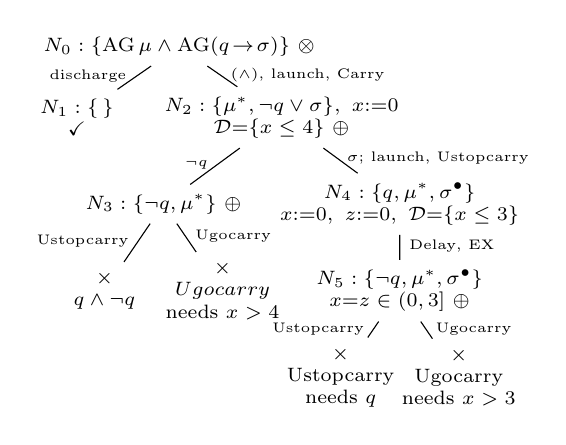
\begin{tikzpicture}[
  every node/.style={align=center, font=\scriptsize},
  level 1/.style={sibling distance=26mm, level distance=9mm},
  level 2/.style={sibling distance=30mm, level distance=11mm},
  level 3/.style={sibling distance=15mm, level distance=11mm},
  level 4/.style={sibling distance=15mm, level distance=11mm},
  edge from parent/.style={draw,-}
]
\node {$N_0:\{\mathrm{AG}\,\mu\wedge\mathrm{AG}(q\!\rightarrow\!\sigma)\}\ \ANDn$}
 child { node {$N_1:\{\,\}$\\ $\OPEN$}
   edge from parent node[left,font=\tiny,pos=.45]{\rl{discharge}} }
 child { node {$N_2:\{\mu^{\ast},\neg q\vee\sigma\},\ x{:=}0$\\ $\Deadline{=}\{x\le 4\}\ \ORn$}
   child { node {$N_3:\{\neg q,\mu^{\ast}\}\ \ORn$}
     child { node {$\CLOSED$\\ $q\wedge\neg q$}
       edge from parent node[left,font=\tiny,pos=.45]{\rl{Ustopcarry}} }
     child { node {$\CLOSED$\\ $\rl{Ugocarry}$\\ needs $x>4$}
       edge from parent node[right,font=\tiny,pos=.45]{\rl{Ugocarry}} }
     edge from parent node[left,font=\tiny,pos=.45]{$\neg q$} }
  child { node {$N_4:\{q,\mu^{\ast},\sigma^\bullet\}$\\ $x{:=}0,\ z{:=}0,\ \Deadline{=}\{x\le3\}$}
     child { node {$N_5:\{\neg q,\mu^{\ast},\sigma^\bullet\}$\\ $x{=}z\in(0,3]\ \ORn$}
       child { node {$\CLOSED$\\ \rl{Ustopcarry} \\needs $q$}
         edge from parent node[left,font=\tiny,pos=.45]{\rl{Ustopcarry}} }
       child { node {$\CLOSED$\\ \rl{Ugocarry} \\needs $x>3$}
         edge from parent node[right,font=\tiny,pos=.45]{\rl{Ugocarry}} }
       edge from parent node[right,font=\tiny,pos=.45]{\rl{Delay}, \rl{EX}} }
     edge from parent node[right,font=\tiny,pos=.4]{$\sigma$; \rl{launch}, \rl{Ustopcarry}} }
   edge from parent node[right,font=\tiny,pos=.45]{$(\wedge)$, \rl{launch}, \rl{Carry}} };
\end{tikzpicture}}
\subcaption{$\mathrm{AG}(\mathrm{AF}_{[1,4]} q)\wedge\mathrm{AG}(q \rightarrow
\mathrm{AG}_{(0,3]}(\lnot q))$.}
\label{fig:ex-roll}
\end{subfigure}
\hfill
\begin{subfigure}[b]{0.48\textwidth}\centering
\resizebox{0.9\linewidth}{!}{%
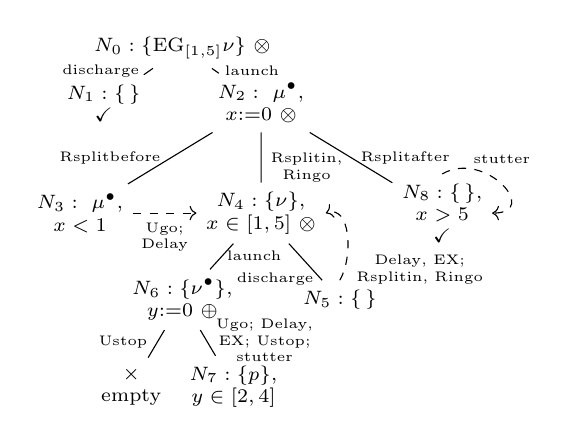
\begin{tikzpicture}[
  every node/.style={align=center, font=\scriptsize},
  level 1/.style={sibling distance=20mm, level distance=7mm},
  level 2/.style={sibling distance=23mm, level distance=14mm},
  level 3/.style={sibling distance=20mm, level distance=11mm},
  level 4/.style={sibling distance=13mm,level distance=11mm},
  edge from parent/.style={draw,-}
]
\node {$N_0:\{\mathrm{EG}_{[1,5]}\nu\}\ \ANDn$}
 child { node {$N_1:\{\,\}$\\ $\OPEN$}
   edge from parent node[left,font=\tiny,pos=.45]{\rl{discharge}} }
 child { node {$N_2:\ \mu^\bullet,$\\$x{:=}0\ \ANDn$}
   child { node (bef) {$N_3:\ \mu^\bullet,$\\$ x<1$}
    edge from parent node[left,font=\tiny,pos=.5]{\rl{Rsplitbefore}} }
   child { node (in) {$N_4:\{\nu\},$\\$ x\in[1,5]\ \ANDn$}
     child { node {$N_6:\{\nu^\bullet\},$\\$ y{:=}0\ \ORn$}
       child { node {$\CLOSED$\\ empty}
         edge from parent node[left,font=\tiny,pos=.45]{\rl{Ustop}} }
       child { node {$N_7:\{p\},$\\$ y\in[2,4]$}
         edge from parent node[right,font=\tiny,pos=.4]{\rl{Ugo}; \rl{Delay},\\ \rl{EX}; \rl{Ustop}; \\stutter} }
       edge from parent node[right,,xshift=-2pt,font=\tiny,pos=.45]{\rl{launch}} }
       child { node (disch) {$N_5:\{\,\}$}
       edge from parent node[left, yshift=-7pt,xshift=7pt,font=\tiny,pos=.45]{\rl{discharge}} }
     edge from parent node[right,font=\tiny,pos=.7]{\rl{Rsplitin},\\ \rl{Ringo}} }
   child { node (aft) {$N_8:\{\,\},$\\$ x>5$\\ $\OPEN$}
     edge from parent node[right,font=\tiny,pos=.5]{\rl{Rsplitafter}} }
   edge from parent node[right,font=\tiny,pos=.45]{\rl{launch}} };
\draw[->,dashed] (bef.east) to[out=0,in=180,looseness=.7]
  node[below,font=\tiny,pos=.5]{\rl{Ugo}; \\\rl{Delay}} (in.west);
\draw[->,dashed] (disch.north) to[out=60,in=20,looseness=1]
  node[right,yshift=-4pt,font=\tiny,pos=.25]{\rl{Delay}, \rl{EX};\\ \rl{Rsplitin}, \rl{Ringo} } (in.east);



\draw[->,dashed] (aft.north) to[out=30,in=0,looseness=2]
  node[above, yshift=4pt,font=\tiny]{stutter} (aft.east);
\end{tikzpicture}}
\subcaption{$\mathrm{EG}_{[1,5]}\tEU{\top}{p}{[2,4]}$.}\label{fig:ex-zeno}
\end{subfigure}
\caption{Two tableau runs. %$\ANDn$ marks an AND-node;$\ORn$ an OR-node. 
$\OPEN$ marks an open node, $\CLOSED$ a closed
one.}\label{fig:ex2}
\end{figure}

%\begin{example}%[A Zeno cycle that may be left]\label{ex:zeno}
Consider $\mathrm{EG}_{[1,5]}\,\nu$, where $\nu=\tEU{\top}{p}{[2,4]}$. Write $x$ for the clock of
the release, and $y$ for that of $\nu$. \ruleref{Cov} splits $N_0$ into a discharge child, which
carries no pursuit, and the launch $N_2$, where $x$ is reset. \ruleref{Rsplit} then partitions the zone,
conjunctively, into its three parts. At $N_3$, the \ruleref{Rsplitbefore} part, \ruleref{Delay} carries $x$ into  \kI. $N_8$, where $x>5$, drops $\mu^\bullet$ and leaves a goal-free node that
may delay indefinitely: a time-progressing loop, since no until needs to be fulfilled and $x$ is
extrapolated above $M$.
\noindent
$N_4$ represents the \ruleref{Rsplitin} part of \ruleref{Rsplit}, where $\nu$ is inserted into $\Gamma$ and so
demanded. \ruleref{Cov} applies, giving two conjunctive branches. The \ruleref{launch} child $N_6$
proves $\nu$. It carries $\nu^\bullet$ with $y$ reset; its \ruleref{Ustop} is empty there, the window
$[2,4]$ not yet open, so only \ruleref{Ugo} survives until a delay carries $y$ into $[2,4]$, where
\ruleref{Ustop} asserts $p$ and drops $\nu^\bullet$. The \ruleref{discharge} child $N_5$ drops $\nu$
from $\Gamma$ and carries $\mu^\bullet$ on; a delay and \ruleref{EX} revive the release, still inside
$[1,5]$, and its in-part demands $\nu$ once more. The search is back at $N_4$, closing a loop. That
loop is not time-progressing: $x$ is never reset, and the in-window zone holds it below $5$.
\noindent
Nonetheless, we can construct a successful marking  as $\mathcal M=\{N_0,\allowbreak N_1,\allowbreak N_2,\allowbreak N_3,\allowbreak N_4,\allowbreak N_5,\allowbreak N_6,\allowbreak N_7,\allowbreak N_8\}$. \ref{M2} holds because the only until pursuit is $\nu^\bullet$, active at $N_6$, and the path to
$N_7$ takes its \ruleref{Ustop} at a node whose zone meets $y\in[2,4]$. \ref{M1} holds because every node of
$\mathcal M$ reaches a time-progressing loop: the nodes carrying the release reach $N_8$ by delaying
until $x$ passes $5$, which lapses it, while $N_1$ and, once $\nu^\bullet$ is dropped, $N_7$ carry
no pursuit, so no deadline caps their delays and their stutter loops are time-progressing. So $\mathcal M$, as well as the tableau, are successful and
$\mathrm{EG}_{[1,5]}\,\nu$ is \SAT.


\section{The Decision Procedure}\label{sec:correct}

Section~\ref{sec:tableau} reduces satisfiability of $\varphi$ to whether $N_0$ lies in a successful
marking of $\TabGraph$. The procedure that decides this rests on reading the conditions of
\S\ref{ss:loop} as a removal operator $F$ on subsets of $\TabNode$. 
%itemjoin={{; }}, itemjoin*={{; and }}
For $A\subseteq\TabNode$, a node
$v\in A$ survives when
\begin{enumerate}[label={\footnotesize\textbf{(D\arabic*)}}, ref={\footnotesize\textbf{(D\arabic*)}},itemindent=2em,
                   ]
\item\label{D1} $v$ is not closed
\item\label{D2} $\ch(v)\cap A\neq\emptyset$ if $\kind(v)=\ORn$, and $\ch(v)\subseteq A$ if
$\kind(v)=\ANDn$
\item\label{D3} $v$ satisfies \ref{M1} and \ref{M2} with its paths taken inside $A$
\end{enumerate}
\noindent
that is, $F(A)=\{v\in A \mid \text{$v$ satisfies \ref{D1}--\ref{D3} on $A$} \}.$ 

$F$ is monotone by construction. Let $A\subseteq B\subseteq\TabNode$ and let $v\in F(A)$. Then
$v\in B$, and each of \ref{D1}--\ref{D3} still holds of $v$ on $B$: \ref{D1} does not mention the
set; a \ORn-node keeps in $B$ the child it had in $A$, and an \ANDn-node has all its children in
$A\subseteq B$; and a path inside $A$ is a path inside $B$, which settles \ref{D3} and \ref{D3}.
Hence $v\in F(B)$ and $F(A)\subseteq F(B)$.


%%%%%%%%% DEAD TEXT %%%%%%%%
% The same operator stated by what it deletes rather than what it keeps; kept in
% case the removal phrasing reads better in the (D3)/(D4) clauses.
%\S\ref{ss:loop} as an operator $F$ which removes from a set $A\subseteq\TabGraph$:
%\begin{enumerate*}[label={\textbf{(D\arabic*)}}, ref={\textbf{(D\arabic*)}},
%                   itemjoin={{; }}, itemjoin*={{; and }}]
%\item the closed nodes
%\item the \ORn-nodes with no child in $A$, and the \ANDn-nodes with a child outside $A$
%\item the nodes at which \ref{M1} fails when its paths are taken inside $A$
%\item the nodes at which \ref{M2} fails when its paths are taken inside $A$.
%\end{enumerate*}
%%%%%%%%% DEAD TEXT %%%%%%%%



%
%Let $A\subseteq B$ and $v\in F(A)$, so $v\in A$ and $v$ survives every clause on $A$. Then
%$v\in B$, and it survives them on $B$ as well: \ref{D1} does not mention the set; a \ORn-node
%keeps its child in $A\subseteq B$; an \ANDn-node has no child outside $A$, and a child outside
%$B$ would be one; and a path inside $A$ is a path inside $B$, which settles \ref{D3} and
%\ref{D4}. So $v\in F(B)$ and $F$ is monotone.

\begin{lemma}\label{prop:gfp}
\TabGraph has a greatest successful marking $\mathcal{M}^*$ and succeeds
iff $N_0\in\mathcal{M}^*$.
\end{lemma}
\begin{proof}
Since $F$ is monotone and $\TabGraph$ is finite by Lemma~\ref{lem:finiteness}, by Knaster--Tarski, $F$ has a greatest fixpoint $\nu F$. Every marking surviving \ref{D1}--\ref{D3} is successful by construction, hence $\nu F$ is the greatest successful marking. As a consequence, the tableau succeeds on $\varphi$ iff $N_0\in\nu F$.
\end{proof}


A procedure that naively iterates $F$ downwards from $\TabGraph$ reaches $\nu F$ in finitely many steps, but presupposes
the full construction of $\TabGraph$. Instead, Algorithm~\ref{alg:otf} decides $N_0\in\nu F$ on-the-fly, building only the part of $\TabGraph$ required. It works by expanding each node of \TabGraph until its children (line~\ref{ln:expand}). Lines~\ref{ln:seed}--\ref{ln:decide} take a strongly
connected component (SCC) $C$ of the expansion whose children outside $C$ are all either in $\Acc$
or $\Rej$, apply $F$ inside $C$, accept what survives and reject the rest (Line~\ref{ln:decide}). $\Acc$ is
passed to $F$ at line~\ref{ln:fix}, so a node of $C$ whose witness leaves $C$ through an accepted
child finds it continued there.
The loop exits once $N_0$ is decided, and $\varphi$ is
satisfiable exactly when $N_0$ ends in $\Acc$. Lines~\ref{ln:acc} and~\ref{ln:rej} are optimizations which allow pruning: a \ORn-node with an accepted child, or an \ANDn-node with
a rejected one, is decided on the spot, so only the components of $E\setminus (\Acc\cup\Rej)$ are ever computed.

\begin{algorithm}[t]
\footnotesize
\DontPrintSemicolon
\SetAlgoLined
\SetAlgoNoEnd
\KwIn{$\varphi$ in negation normal form}
\KwOut{\SAT{} or \UNSAT}
$E\gets\{N_0\}$; \quad $\Acc\gets\emptyset$; \quad $\Rej\gets\emptyset$\label{ln:init}\;
\Repeat{$N_0\in \Acc \cup \Rej$\label{ln:until}}{
  $\Acc\gets\Acc\cup\{v\in E\mid \kind(v)=\ORn,\ \ch(v)\cap\Acc\neq\emptyset\}$\label{ln:acc}\;
  $\Rej\gets\Rej\cup\{v\in E\mid \kind(v)=\ANDn,\ \ch(v)\cap\Rej\neq\emptyset\}$\label{ln:rej}\;
  \ForEach{component $C$ of $E\setminus (\Acc\cup\Rej)$ with $\ch(C)\setminus C\subseteq \Acc\cup\Rej$\label{ln:comp}}{
    $X\gets C$\label{ln:seed}\;
    \lRepeat{$X$ \textnormal{is unchanged}}{$X\gets F(X\cup\Acc)\cap C$\label{ln:fix}}
    $\Acc\gets\Acc\cup X$; \quad $\Rej\gets\Rej\cup(C\setminus X)$\label{ln:decide}\;
  }
  $E\gets E\cup\ch(E\setminus (\Acc\cup\Rej))$\tcp*{apply the rules of \S\ref{ss:rules}}\label{ln:expand}
}
\Return{\SAT{} \textnormal{if} $N_0\in\Acc$, \textnormal{else} \UNSAT}\label{ln:return}
\caption{Satisfiability check for TCTL formula $\varphi$}\label{alg:otf}
\end{algorithm}

Correctness of the procedure rests on three further facts: \ref{lemitem:pruning} pruning preserves $\nu F$; \ref{lemitem:de} a time-progressing cycle is found by inspecting resets and bounds, making \ref{D3} computable; and \ref{lemitem:fix} $F$ may be applied inside a single component, preserving the greatest fixpoint and allowing for an on-the-fly decision.

\begin{lemma}\label{lem:search}
$A\subseteq\mathcal M^{*}$ be a successful marking with $\mathcal M^{*}\cap(\ch(C)\setminus C)\subseteq A$.
\begin{enumerate}[label=\emph{(\roman*)}, ref={(\roman*)}]
\item\label{lemitem:pruning} If $v$ is a \ORn-node with a child $w\in\mathcal M^{*}$, or an
\ANDn-node with a child $w\notin\mathcal M^{*}$, then $v\in\mathcal M^{*}$ iff
$w\in\mathcal M^{*}$. Removing $v$'s other children leaves $\mathcal M^{*}$ unchanged.
\item\label{lemitem:de} $T$ contains a time-progressing cycle iff some node of $T$ is a
\ruleref{Delay}-successor and every clock is unbounded or reset in $T$.
\item\label{lemitem:fix} $\mathcal M^{*}\cap C$ is the largest $X\subseteq C$ with
$X\subseteq F(X\cup A)$.
\end{enumerate}
\end{lemma}
\begin{proof}
\ref{lemitem:pruning} For an \ANDn-node this is \ref{D2}. For a \ORn-node, $\mathcal M^{*}\cup\{v\}$
is a post-fixpoint of $F$: $v$ is not closed and spared by \ref{D2} because of $w$; and \ref{D3} hold at $v$ by prefixing the edge
$v\to w$ to the witnesses $w$ carries, a pursuit active at $v$ being either still active at $w$ or
discharged by that edge. Hence $v\in\nu F=\mathcal M^{*}$. The same prefixing gives the second
claim: a path using another child of $v$ arrives through $v$, so a node relying on it can take its
own path to $v$ and then $v$'s witness. \ref{lemitem:de} ($\Leftarrow$) Strong connectivity gives a cycle through the
\ruleref{Delay}-successor and a reset node of each clock $T$ resets, which is then
time-progressing. ($\Rightarrow$) By definition a time-progressing cycle elapses positive time, so it crosses a \ruleref{Delay}, since it is the only rule that elapses time, and every clock is either reset on it or extrapolated above $M$, hence unbounded. 
\ref{lemitem:fix} For $\subseteq$, $C$ being maximal a witness path of $\mathcal M^{*}$ from
$N\in C$ either stays in $C$ or leaves once through some $c\in A$, where it continues since $A$ is a
successful marking. For $\supseteq$, $X\cup A$ is then a successful marking too, its $A$-part by
monotonicity and its $X$-part by hypothesis, so $X\subseteq\mathcal M^{*}$ by
Proposition~\ref{prop:gfp}.
\end{proof}

\begin{theorem}\label{thm:alg}
Algorithm~\ref{alg:otf} terminates in $2^{\mathrm{poly}(n)}$ and returns \SAT{} iff $N_0\in\nu F$.
\end{theorem}



\begin{proof}
Let $D=\Acc\cup\Rej$ and $U=E\setminus D$. Each iteration enlarges $E$ or $D$, or the loop exits.
Suppose one enlarges $D$ by nothing; then $E$, $D$ and $U$ still carry the values they had on
entry when line~\ref{ln:expand} runs. If $U=\emptyset$ then $E=D$, so $N_0\in D$ and the loop
exits. Otherwise suppose line~\ref{ln:expand} adds nothing either, that is $\ch(U)\subseteq E$.
The condensation of the subgraph induced on $U$ is non-empty, finite and acyclic, so it has a sink
$C$: a maximal SCC of $U$ with $\ch(C)\cap U\subseteq C$. Take any $w\in\ch(C)\setminus C$. It
lies outside $U$ by sinkhood, and inside $E$ by that supposition, hence in $D$. So every exit of
$C$ is decided, $C$ meets the guard of line~\ref{ln:comp}, and line~\ref{ln:decide} adds the
non-empty $C$ to $D$, against the assumption that $D$ did not grow. Hence
$\ch(U)\not\subseteq E$, and line~\ref{ln:expand} enlarges $E$. Both sets are bounded by $|\TabNode|$, finite by Lemma~\ref{lem:finiteness}, so at most
$2|\TabNode|$ iterations enlarge either and the next one exits, necessarily with $N_0\in D$ as
that is the guard of line~\ref{ln:until}.



We show $\Acc\subseteq\mathcal M^{*}$ and $\Rej\cap\mathcal M^{*}=\emptyset$ by induction on the
order in which nodes are accepted or rejected, each such step resting on those already taken.
Lines~\ref{ln:acc} and~\ref{ln:rej} are Lemma~\ref{lem:search}\ref{lemitem:pruning}, which also
justifies leaving the remaining children unbuilt. Line~\ref{ln:comp} fires only once every child
of $C$ outside $C$ has been accepted or rejected, so by induction
$\Acc\cap\ch(C)=\mathcal M^{*}\cap(\ch(C)\setminus C)$; line~\ref{ln:fix} then computes
$\mathcal M^{*}\cap C$ by Lemma~\ref{lem:search}\ref{lemitem:fix}, and line~\ref{ln:decide}
accepts it and rejects the rest of $C$. Clause~\ref{D3} of $F$ is evaluated through
Lemma~\ref{lem:search}\ref{lemitem:de}.

For the bound let $m$ be that of Lemma~\ref{lem:finiteness}; as $M$
occupies at most $n$ input symbols, $\log m=O(n)+O(n^{2})\log M=\mathrm{poly}(n)$, and each of the at
most $2m$ rounds costs one decomposition of a subgraph of $\TabGraph$ together with at most $m$
applications of $F$, each a decomposition and $O(n)$ backward reachabilities linear in the subgraph,
so the run costs $\mathrm{poly}(m)=2^{\mathrm{poly}(n)}$.
\end{proof}






\section{Soundness and Completeness}\label{ss:sound}
We now prove the procedure is sound, i.e., that if the tableau succeeds on $\varphi$, then $\varphi$ is \SAT, and complete for non-punctual TCTL, i.e., that if $\varphi$ is \SAT, then the tableau succeeds on $\varphi$. These results are supported by the following lemma.
\begin{lemma}\label{lem:zones}
Let $N_0,\dots,N_k$ be a path of $\TabGraph$ with non-empty zones.
\begin{enumerate*}[label=\emph{(\roman*)}, ref={(\roman*)}, itemjoin={{\ }}, itemjoin*={{\ }}]
\item\label{zoneitem:feasible} For every $\nu_k\in Z_k$ there are $\nu_i\in Z_i$ and delays realising
every step, positive at every \ruleref{Delay} step.
\item\label{zoneitem:stability} If a delay crosses no integer hyperplane $x=b$ with $b\le M$, every
subformula of $\varphi$ has constant truth on the open segment it sweeps.
\item\label{zoneitem:nonzeno} A cycle of $\TabGraph$ has a non-Zeno unfolding iff it is
time-progressing, and then one whose iterations elapse a constant positive amount.
\end{enumerate*}
\end{lemma}
\begin{proof}
\ref{zoneitem:feasible} Every zone operation a rule performs (intersection with a guard, reset, time-successor,
$\cong_M$-canonicalisation) admits back-propagation, non-empty precisely because the successor
valuation lies in its image~\cite{Bouyer05TimedAutomata}; thread backwards from $\nu_k$, the delay of
a \ruleref{Delay} step being positive since $\Dopen Z$ and $\Dbd Z$ lie strictly ahead of $Z$.
\ref{zoneitem:stability} No clock crosses an integer at or below $M$, so no integer part changes and no
fractional ordering wraps, while clocks above $M$ are identified by extrapolation; the segment lies in
one clock region, on which TCTL truth is
constant~\cite{AlurCourcoubetisDill1990,Bouyer05TimedAutomata}, and its endpoints are nodes of their
own by the integer split of \ruleref{Delay}.
\ref{zoneitem:nonzeno} By contraposition, a cycle elapsing no time takes zero time over any number of
traversals; and if some clock is neither reset on it nor extrapolated above $M$, it keeps a bound
$c\le M$, grows by exactly the delay elapsed, and caps the total at $c$. Conversely \ref{zoneitem:feasible} yields
a traversal elapsing some $\delta>0$, and the cycle returning to its first node, no rule distinguishes
two visits and no clock depletes a budget, so $\delta$ recurs at every iteration.
\end{proof}

\subsection{Soundness}\label{subsec:soundness}


In order to prove soundness, we proceed by constructing a witness automaton $\mathcal A_\varphi$ from a successful marking $\mathcal M^{*}$ of the tableau graph $\TabGraph$. We then show that this automaton satisfies the formula $\varphi$.

The construction is straightforward. The saturated nodes of $\mathcal M^{*}$ supply the locations
$S$ of $\mathcal A_\varphi$: a saturated $N$ carries $L(N)=\Gamma_{\mathsf{prop}}$ and
$\mathsf{Inv}(N)$, and $N_0$ is the initial location. Every \ruleref{Delay}- or
\ruleref{EX}-child of $N$ that $\mathcal M^{*}$ retains supplies an outgoing edge of $E$, leading
to the next node and carrying the reset clocks, i.e., $x_\mu$ at a \ruleref{launch} and at a \ruleref{Ustopcarry}. Those rules
elapse no time and leave $L$ and $\mathsf{Inv}$ untouched, so they contribute no edge of their own.

Each location carries a schedule, which follows the finite path of $\mathcal M^{*}$ discharging one of the at most $n+1$ obligations pending there, resolving the \ORn-nodes along that path and turning round-robin to the next obligation once the current one is discharged. Its memory is the pair (obligation, position on that path), so $S$ stays finite.

%
%\ref{M1} and \ref{M2} hold of a path, however, and a
%location must commit to one, so it carries in addition a \emph{schedule}. At most $n+1$
%obligations are pending at $N$, the divergence of \ref{M1} and the until pursuits active there, and
%each is discharged by a finite path of $\mathcal M^{*}$; the schedule follows one such path,
%resolving the \ORn-nodes along it, and turns round-robin to the next obligation once the current one
%is discharged. Its memory is the pair (obligation, position on that path), so the locations stay
%finite.
%
%
%\ref{M1} and \ref{M2} promise one path of $\mathcal M^{*}$ per obligation, though, while a run of
%$\mathcal A_\varphi$ commits to one branch at every \ORn-node, and no single branch serves every
%obligation: under $\mathrm{AG}(\mathrm{EF}\,p\wedge\mathrm{EF}\,q)$ a node must head for $p$ on some
%visits and for $q$ on others. A location therefore pairs a saturated node with a \emph{schedule},
%which follows the finite path discharging one of the at most $n+1$ obligations pending there, the
%divergence of \ref{M1} and the until pursuits active at it, resolving the \ORn-nodes along that
%path and turning round-robin to the next obligation once the current one is discharged. Its memory
%is the pair (obligation, position on that path), so $S$ stays finite.
%

%
%Call a node of $\mathcal M^{*}$ a \emph{state} if it is
%saturated, so that its children are the successor steps; the remaining, \emph{expansion} edges
%neither elapse time nor change location, and reset a clock only through a \ruleref{launch} or a
%\ruleref{Ustopcarry}. At most $n+1$ obligations are pending at $N$, the divergence requirement of
%\ref{M1} and the until pursuits active there, and \ref{M1}, \ref{M2} give a finite path $\pi_{N,o}$
%of $\mathcal M^{*}$ discharging each. A \emph{schedule} selects at every \ORn-node the child
%$\pi_{N,o}$ prescribes and moves round-robin to the next pending obligation once $o$ is discharged,
%so its memory, the pair (obligation, position on $\pi_{N,o}$), is finite. The witness
%$\mathcal A_\varphi$ has as locations the pairs (state, schedule memory), labelled by
%$\Gamma_{\mathsf{prop}}$ and carrying $\Inv(N)$, and as edges the scheduled successor steps, guarded
%by the zone of the next state reached through expansion edges and resetting the clocks that segment
%resets.
%
\begin{lemma}[Recurrence]\label{lem:recurrence}
Let $\mu=\mathrm{A}(\varphi\,\mathbf{U}_\kI\,\psi)$ with $a=\inf\kI$, $b=\sup\kI<\infty$, and let
$\rho$ be a run of $\mathcal A_\varphi$ through a node carrying $\mu^{\ast}$, launched at $t_0$. Then
\ruleref{Ustopcarry} fires on $\rho$ at times $t_0<w_1<w_2<\cdots$ with $w_1-t_0\in\kI$ and
$w_{j+1}-w_j\le b-a$, and $\rho\models\varphi\,\mathbf{U}_\kI\,\psi$ from every position at or after
$t_0$.
\end{lemma}
\begin{proof}
No rule drops $\mu^{\ast}$: \ruleref{Ustopcarry} keeps it in $\Gamma$, \ruleref{Ugocarry} moves
$\AX\mu^{\ast}$ to $\Ctx$, whence every successor carries it again, and \ruleref{Absorb} bars a fresh
\ruleref{Cov} while the pursuit is live. So $\mu^{\ast}$ rides $\rho$ for ever, and with it the
deadline on $x_\mu$, which is $b$ until the first witness and $b-a$ after. Both are at most $M$, so
$x_\mu$ is bounded along $\rho$, and a cycle leaving a bounded clock unreset is not
time-progressing. By \ref{M1} the schedule reaches such a cycle and traverses it without end, and
while the pursuit is live only \ruleref{Ustopcarry} resets $x_\mu$, so the stop recurs: it fires at
times $t_0<w_1<w_2<\cdots$. At the first firing $x_\mu$ measures from $t_0$ and the guard is \kI, so
$w_1-t_0\in\kI$; at each later one it measures from the preceding witness and $\Deadline$ caps it at
$b-a$, so $w_{j+1}-w_j\le b-a$.

For the last claim let $t\ge t_0$ and let $w_j$ be the first witness at or after $t+a$. If $j=1$ then
$w_1\le t_0+b\le t+b$; otherwise $w_{j-1}<t+a$, so $w_j\le w_{j-1}+(b-a)<t+b$. Either way
$w_j-t\in\kI$, and $\psi$ holds at $w_j$ while \ruleref{Ugocarry} asserts $\varphi$ at every position
before it, which is \eqref{eq:sat_u}.
\end{proof}

\begin{theorem}\label{thm:soundness}
If Algorithm~\ref{alg:otf} returns \SAT{} then $\varphi$ is satisfiable.%, %and $\mathcal A_\varphi$ is a witness for it.
\end{theorem}
\begin{proof}
By Theorem~\ref{thm:alg} the root lies in $\mathcal M^{*}$, so $\mathcal A_\varphi$ is defined, and
Lemma~\ref{lem:zones}\ref{zoneitem:feasible} supplies valuations and delays along its paths. It is non-blocking: its only
invariants are the deadlines in $\Deadline$, and cap and stop guard derive from the same interval with the
same strictness, so the stop edge is enabled up to the cap and by \ref{M2} the schedule takes it. By
\ref{M1} the schedule reaches a time-progressing cycle, which Lemma~\ref{lem:zones}\ref{zoneitem:nonzeno} unfolds into
a run whose iterations each elapse a fixed $\delta>0$, so $\mathrm{Runs}^\infty$ is non-empty
everywhere, which is all the semantics asks of it.

We show $\mathcal T,(s_0,\mathbf 0)\models\varphi$ for the induced TTS by induction on $\varphi$
along the marking. Propositional goals hold by saturation and closure of contradictory nodes;
$\EX\psi$ obtains a successor satisfying $\psi$ from its \ruleref{EX} child, and $\AX\psi$ holds at
all successors since each child inherits $\Ctx$. For a timed modality demanded at $N$,
\ruleref{Cov} is conjunctive, so $\mathcal M^{*}$ retains both the discharge child, carrying the
remaining goals, and the launch, which establishes $\mu$ with $x_\mu$ reset, so \kI is measured
from this configuration and the pursuit rides every successor, as a goal under $\mathrm{E}$ and as
context under $\mathrm{A}$. A re-demand is covered anew, carried or absorbed, so every onset is established: by a pursuit
of its own, by the carried pursuit that answers all of them, or, when the window is unbounded, by
the witnesses that later launches are forced to produce. An existential until is witnessed by the path \ref{M2} supplies, extended past
its \ruleref{Ustop} by a divergent run; a universal one cannot be evaded, $\Inv(N)$ blocking time at
the cap while the pursuit is imposed on all successors, and when the demand is persistent this is
Lemma~\ref{lem:recurrence}. \ruleref{Rsplit} discharges a release by partitioning the zone
conjunctively: \ruleref{Runf} asserts $\psi$ in the window until $\varphi$ releases it, carries the
pursuit on before the window, and past it the obligation has lapsed.
Lemma~\ref{lem:zones}\ref{zoneitem:stability} lifts each conclusion to the positions between nodes.
\end{proof}

\begin{theorem}[Completeness]\label{thm:completeness}
If $\varphi$ is non-punctual and satisfiable then Algorithm~\ref{alg:otf} returns \SAT.
\end{theorem}
\begin{proof}
Completeness goes the other way: the realisable nodes of \S\ref{ss:nodes} are themselves a successful
marking. Writing $\mathcal R$ for them, we show $\mathcal R\subseteq F(\mathcal R)$; then $\mathcal R\subseteq\mathcal M^{*}$ by
Proposition~\ref{prop:gfp}, and $N_0\in \mathcal R$ as $\varphi$ is satisfiable, so Theorem~\ref{thm:alg}
returns \SAT.

\ref{D1}: a realisable node has a non-empty zone and a consistent $\Gamma_{\mathsf{prop}}$, and
\ruleref{Umiss} does not fire on it: a pending $\mu^\bullet$ is realisable at no valuation beyond
its window, so its zone meets $x_\mu\le b$.
\ref{D2}: let $N\in \mathcal R$ be realised by $\mathcal T$. All children of an \ANDn-rule are realised by the
same $\mathcal T$: \ruleref{Cov} because $\mathcal T$ satisfies $\Gamma\setminus\{\mu\}$ and $\mu$
alike, \ruleref{Rsplit} because its children partition $Z_N$ and realisability is monotone under
narrowing, \ruleref{Delay} and \ruleref{EX} because $\mathcal T$ admits the passage of time and
supplies a successor for every $\EX\psi$, each inheriting $\Ctx$. At an \ORn-rule $\mathcal T$ selects
a child: a disjunct it satisfies for \ruleref{Disj}; for \ruleref{Uunf} and \ruleref{Uunfcarry} the
stop if $\psi$ holds now with $x_\mu\in\kI$ and \ruleref{Ugo} otherwise, the witness being later and
$\varphi$ holding now; for \ruleref{Runf} the stop if $\varphi$ has
released the obligation and the recursive child otherwise. The zone operations being exact, no chosen
zone is empty. A demand re-imposed at a continuum of onsets is answered onset by onset, every re-demand being
covered anew, carried or absorbed according to whether the running pursuit reaches the new onset,
so the selections above serve each onset of each zone.
\ref{D3}: fix $N\in \mathcal R$ and a run $\rho$ of $\mathcal T$ from a configuration for $N$. It
is non-Zeno, so no clock stays both unreset and bounded along it, and following $\rho$ through the
choices above gives a path of $\mathcal R$ from $N$ which by Lemma~\ref{lem:finiteness} repeats a node; that
segment elapses positive time with every clock reset on it or extrapolated above $M$, hence is a
time-progressing cycle of $\mathcal R$ reached from $N$. An until pursuit active at $N$ is one $\mathcal T$
fulfils at a finite position of $\rho$, which the path following $\rho$ carries it to.

Non-punctuality enters at the repetition step: a node summarises the pending obligations of a
persistent universal until by $x_\mu$ alone, the time since the last witness capped at $b-a$, and by
Lemma~\ref{lem:recurrence} that summary is faithful exactly when witnesses spaced at most $b-a$ apart
answer every onset, which needs $b>a$.
\end{proof}


\begin{corollary}\label{cor:depthone}
Satisfiability of non-punctual TCTL is \textsc{ExpTime}-complete, and the procedure is sound and
complete for TCTL of temporal nesting depth at most one, punctual intervals included.
\end{corollary}
\begin{proof}
Membership is Theorems~\ref{thm:alg}--\ref{thm:completeness}; hardness is inherited from CTL
satisfiability~\cite{Clarke99} by fixing every interval to $[0,\infty)$. At depth one every argument
is propositional, so no modality is demanded inside the pursuit of another and no fresh onset arises;
the obligations live at a node are exactly the pursuits it carries, recorded in $\Gamma$, $\Ctx$ and
$\Deadline$ with their elapsed time in $Z$, so a repeat agrees on the full obligation state and
Theorem~\ref{thm:completeness} goes through for every \kI.
\end{proof}

\noindent
Depth one covers reachability, safety and inevitability, the queries
\textsc{Uppaal}~\cite{BehrmannLarsenYi2004Uppaal} and \textsc{Romeo}~\cite{lime-TACAS-09} are asked
for; the one common query beyond it, leads-to $\mathrm{AG}(p\rightarrow\mathrm{AF}_\kI q)$, stays
covered by Theorem~\ref{thm:completeness} whenever \kI is non-punctual.


\section{Evaluation}\label{sec:eval}

We evaluate the procedure through two research questions.

\begin{enumerate}[start=1,label={\bfseries RQ\arabic*:}, itemindent=2em, ref=\bfseries RQ\arabic*, itemsep=0.1em]
\item \label{rq:structural} Which parameters of the input formula drive the cost of the search, and
how does it scale in each?
\item \label{rq:practicality} Is the procedure practical on the flat, one-level TCTL queries
engineers write for \textsc{Uppaal}?
\end{enumerate}

\noindent
\ref{rq:structural} asks where the \textsc{ExpTime} bound of Theorem~\ref{thm:alg} is felt and where
it is not; \ref{rq:practicality} asks the complementary question, whether the queries a specification
is actually checked against lie in the expensive regime.

\paragraph{Benchmark and method.}
No standard suite exists for TCTL \emph{satisfiability}, and there is no second implementation to
compare against, so the study characterises one procedure rather than ranking two. We generate $333$
parameterised instances. For \ref{rq:structural} each family varies a single term of
$2^{O(n)}\cdot M^{O(n^{2})}$ with the others fixed: the number of \emph{simultaneously live}
formula-clocks $k$, obtained by conjoining $k$ independent timed untils; the \emph{nesting depth} $d$
of a timed double-check; the largest constant $M$, swept by powers of two to $2^{20}$; and the
propositional \emph{size} $m$. Each ships matched satisfiable and unsatisfiable variants, so witness
cost and refutation cost are separated. For \ref{rq:practicality} we generate the canonical
\textsc{Uppaal} shapes over atomic propositions, each swept along payload size $m\le1024$ and time
bound $b\le2^{20}$.

We report the number of tableau \emph{nodes} as the primary measure. It is a deterministic function
of the formula, independent of the machine, and it is what Lemma~\ref{lem:finiteness} bounds; every
growth law below is fitted to it. Wall-clock time and peak resident memory are reported as maxima
only. Each instance was given $600$\,s and a $10$\,GB resident-memory cap, run serially on an
Apple~M4~Pro; timing is the median of three runs for instances under $5$\,s and a single run above.
\textbf{No instance timed out, and none reached the memory cap.}

\begin{table}[t]\centering
\caption{\textbf{\ref{rq:structural}: cost drivers.} One row per family and verdict, over the whole sweep.
The growth law is fitted to the \emph{node count}, which is a deterministic function of the formula;
wall-clock is reported as a maximum only, since instrumentation floors it at $0.2$\,s. No instance
timed out or reached the memory cap.}\label{tab:rq1}
\small\setlength{\tabcolsep}{5pt}
\begin{tabular}{llccrrrr}
\toprule
Factor & Verdict & Range & Nodes & $R^2$ & max nodes & max $t$\,(s) & max mem\,(MB)\\
\midrule
Clocks $k$ & SAT & 1--20 & $\mathbf{1.93^{k}}$ & 1.00 & 4{,}194{,}836 & 494.57 & 3628 \\
Clocks $k$ & UNSAT & 1--20 & linear & 0.99 & 279 & 0.20 & 2 \\
Depth $d$ & UNSAT & 1--12 & $d^{2.48}$ & 1.00 & 211{,}527 & 11.16 & 178 \\
Depth $d$ & SAT & 1--12 & $d^{1.84}$ & 0.98 & 10{,}283 & 0.49 & 9 \\
Size $m$ & SAT & 1--1024 & $m^{0.63}$ & 0.94 & 1{,}038 & 0.82 & 32 \\
Const $M$ & SAT & 2--1048576 & flat & --- & 286 & 0.20 & 4 \\
Const $M$ & UNSAT & 1--1048576 & flat & --- & 401 & 0.20 & 2 \\
\bottomrule
\end{tabular}
\end{table}


\paragraph{\ref{rq:structural}: one exponential driver, and it is not nesting.}
Table~\ref{tab:rq1} ranks the four factors, and they separate sharply.

\emph{Clock simultaneity is the only exponential axis.} On satisfiable instances the node count is
$1.93^{k}$ with $R^{2}=1.00$ over the whole sweep $k=1..20$, a clean doubling per added clock, ending
at $4.19$M nodes, $3.6$\,GB and $495$\,s. This is the $M^{O(n^{2})}$ handle: $k$ clocks live at once
means a DBM of dimension $k+1$, and a witness has to meet all $k$ windows together, so the search
enumerates their product.

\emph{Nesting depth is polynomial.} Refutation grows as $d^{2.48}$ ($R^{2}=1.00$) and a witness as
$d^{1.84}$, so depth~$12$ costs $211$k nodes and $11$\,s unsatisfiable, $10$k nodes and half a second
satisfiable. Nesting is an order of magnitude cheaper than the bound permits, because the memoised
graph collapses the repeated structure of the nested check instead of unfolding it.

\emph{Neither $M$ nor formula size is a driver.} The node count is constant at $293$ across six
orders of magnitude of $M$, from $1$ to $2^{20}$: a zone represents a large bound symbolically, and
$\cong_M$ leaves the realised set identical. Propositional size is sublinear, $m^{0.63}$, so a
payload of $1024$ atoms realises $1038$ nodes. The closure grows; the search does not.

\emph{The witness/refutation asymmetry runs in both directions,} and which way depends on what the
formula demands. On clocks the satisfiable side is the expensive one, $4.19$M nodes against $279$: a
model must meet every obligation at once, whereas a single contradiction closes the refutation
outright. On depth the order reverses, $211$k against $10$k: the witness is short-circuited at the
first accepting branch, while the refutation has to exhaust the graph. The ranking is therefore
$\textit{clocks}\gg\textit{depth}\gg\{M,\textit{size}\}$, with the exponential confined to
satisfiable instances of the first.

\begin{figure}[t]\centering
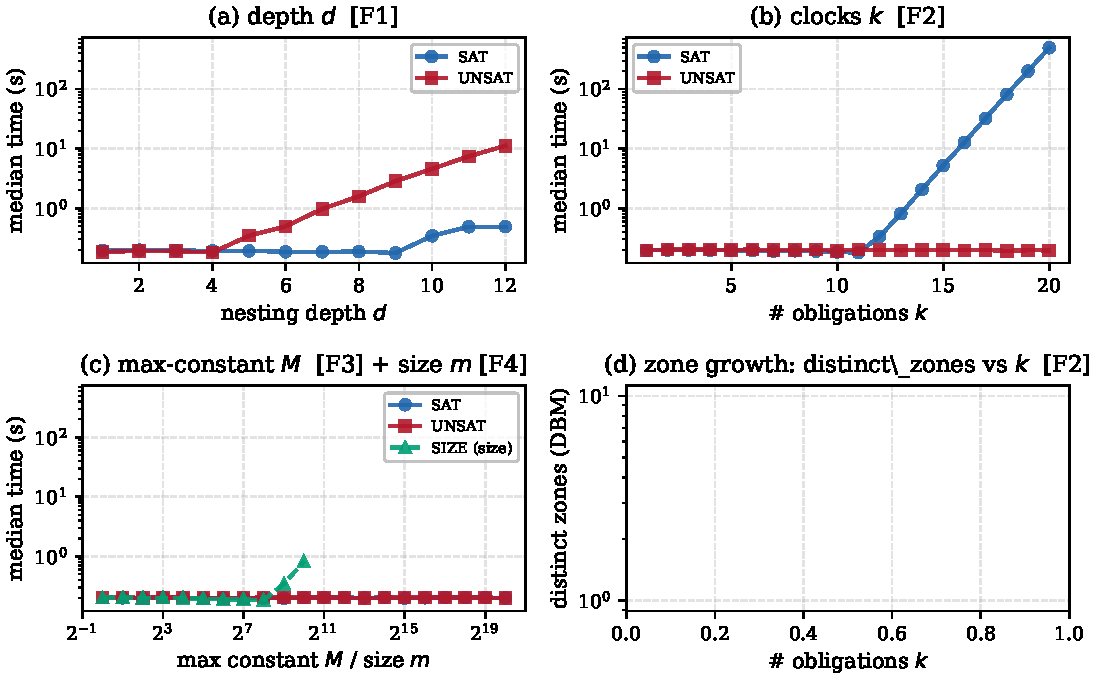
\includegraphics[width=0.72\textwidth]{figs/fig_drivers.pdf}
\caption{\ref{rq:structural} cost drivers: median runtime against each parameter, satisfiable and
unsatisfiable shown separately. Clock simultaneity is exponential, depth is polynomial, and the
constant $M$ and the propositional size are flat.}\label{fig:drivers}
\end{figure}

\begin{table}[t]\centering
\caption{\textbf{\ref{rq:practicality}: the \textsc{Uppaal} query shapes.} Worst case over the full
sweep of payload size $m\in[1,1024]$ and time bound $b$, per shape. All $217$ instances were solved;
none timed out.}\label{tab:rq2}
\small\setlength{\tabcolsep}{5pt}
\begin{tabular}{llcrrrr}
\toprule
Shape & TCTL form & $b$ range & \# & max nodes & max $t$\,(s) & max mem\,(MB)\\
\midrule
Reachability & $\mathrm{EF}_{[0,b]}\,\Phi$ & 1--$2^{20}$ & 52 & 1{,}030 & 0.50 & 27 \\
Safety & $\mathrm{AG}_{[0,b]}\,\Phi$ & 1--$2^{20}$ & 52 & 3{,}091 & 0.51 & 28 \\
Bounded liveness & $\mathrm{AF}_{[1,b]}\,\Phi$ & 2--$2^{20}$ & 51 & 1{,}038 & 0.51 & 27 \\
Leads-to & $\mathrm{AG}(p\!\rightarrow\!\mathrm{AF}_{[1,b]}q)$ & 2--$2^{20}$ & 51 & 15{,}489 & 1.14 & 39 \\
Possibly-always & $\mathrm{EG}_{[0,\infty)}\,\Phi$ & --- & 11 & 2{,}059 & 0.82 & 33 \\
\bottomrule
\end{tabular}
\end{table}


\paragraph{\ref{rq:practicality}: the queries engineers write are far from the wall.}
All $217$ instances of the \textsc{Uppaal} sweep are solved, none times out, and the worst case over
every shape and both axes is $1.14$\,s, $15{,}489$ nodes and $39$\,MB (Table~\ref{tab:rq2}). The time
bound is absorbed entirely: swept to $b=2^{20}$, the hardest shape realises $1242$ nodes and stays at
the $0.2$\,s floor, which is the constant-independence of \ref{rq:structural} showing up again. Only
the payload size moves anything, and mildly. Leads-to,
$\mathrm{AG}(p\rightarrow\mathrm{AF}_{[1,b]}q)$, is the costliest shape by an order of magnitude in
nodes, as its nesting depth of two predicts, and is still solved in about a second. Why these shapes
are cheap is visible in \ref{rq:structural}: each keeps one formula-clock live, so the one
exponential axis is never entered.

\paragraph{Threats to validity.}
The benchmark is synthetic; the \textsc{Uppaal} family mitigates this over the canonical query
\emph{shapes}, but on abstract propositions rather than ones drawn from deployed models. No wall was
located: with no timeouts, the largest costs reported are the ends of the sweeps rather than limits
of the procedure, and the $1.93^{k}$ law puts $k\approx24$ past the memory cap. Wall-clock below
$0.2$\,s is dominated by process startup and by the $150$\,ms sampling interval of the memory
watchdog, which is why the fits use node counts; that watchdog also makes the cap a sampled bound
rather than a hard one, macOS implementing no address-space limit. Timings come from one machine and
one zone backend, and the generator, solver and a reproducibility manifest accompany the paper.


\bibliographystyle{splncs04}
\bibliography{ETAPS2026}

\end{document}
